%************************************************
\chapter{Risultati e discussione}\label{ch:risultati}
%************************************************

% ***********************************************
% [ ] Mettere i grafici con le tre classi
% ***********************************************

Per l'implementazione dell'algoritmo è stato scelto il ben noto 
data set Iris, una tabella compilata con lunghezze e larghezze 
del petalo e del sepalo di tre specie di fiore Iris: 
setosa, versicolor e virginica.  
Come evidenziato in Schuld et al. \cite{schuld}, 
l'insieme dati si è dovuto standardizzare e 
normalizzare prima dell'utilizzo. 

% *****************************************
% Questa parte può andare dopo
% *****************************************

% Questa versione esemplificativa è stata fatta girare con successo 
% sul processore quantistico a 5 qubit messo a disposizione dall'IBM.
% Di fronte alla disponibilità di un nuovo computer quantistico a 16 
% qubit\footnote{\url{https://developer.ibm.com/dwblog/2017/quantum-computing-16-qubit-processor/}, 
% Recuperato l'8 settembre 2019}, 
% ci si chiede quali sono le prossibilità di miglioramento delle 
% implementazioni pratiche. Si è lavorato sulle seguenti proprietà: 

% Per fare ciò, si è dovuto tenere in considerazione i compromessi 
% in termini di numero di qubit ed efficienza di classificazione: 
% infatti, per realizzare ognuno di questi punti c'è bisogno di impegnare 
% più qubit, non solo per una questione di memoria, ma anche per 
% la complessità delle operazioni da effettuare; un'esempio è dato 
% dalla porta $C^n R_y (\theta)$, usata nel procedimento di costruzione 
% della \ac{QRAM} (vedi sezione \ref{sec:ff-qram}), che necessita di un 
% qubit ancilla in più per ogni qubit di controllo aggiuntivo. 

\section{Preparazione dei dati}

Il data set Iris completo si presenta nella forma mostrata in figura 
\ref{fig:iris_grezzi}, dove sono graficate due delle quattro caratteristiche 
del data set sugli assi coordinati. 

\begin{figure}[ht]
    \centering
    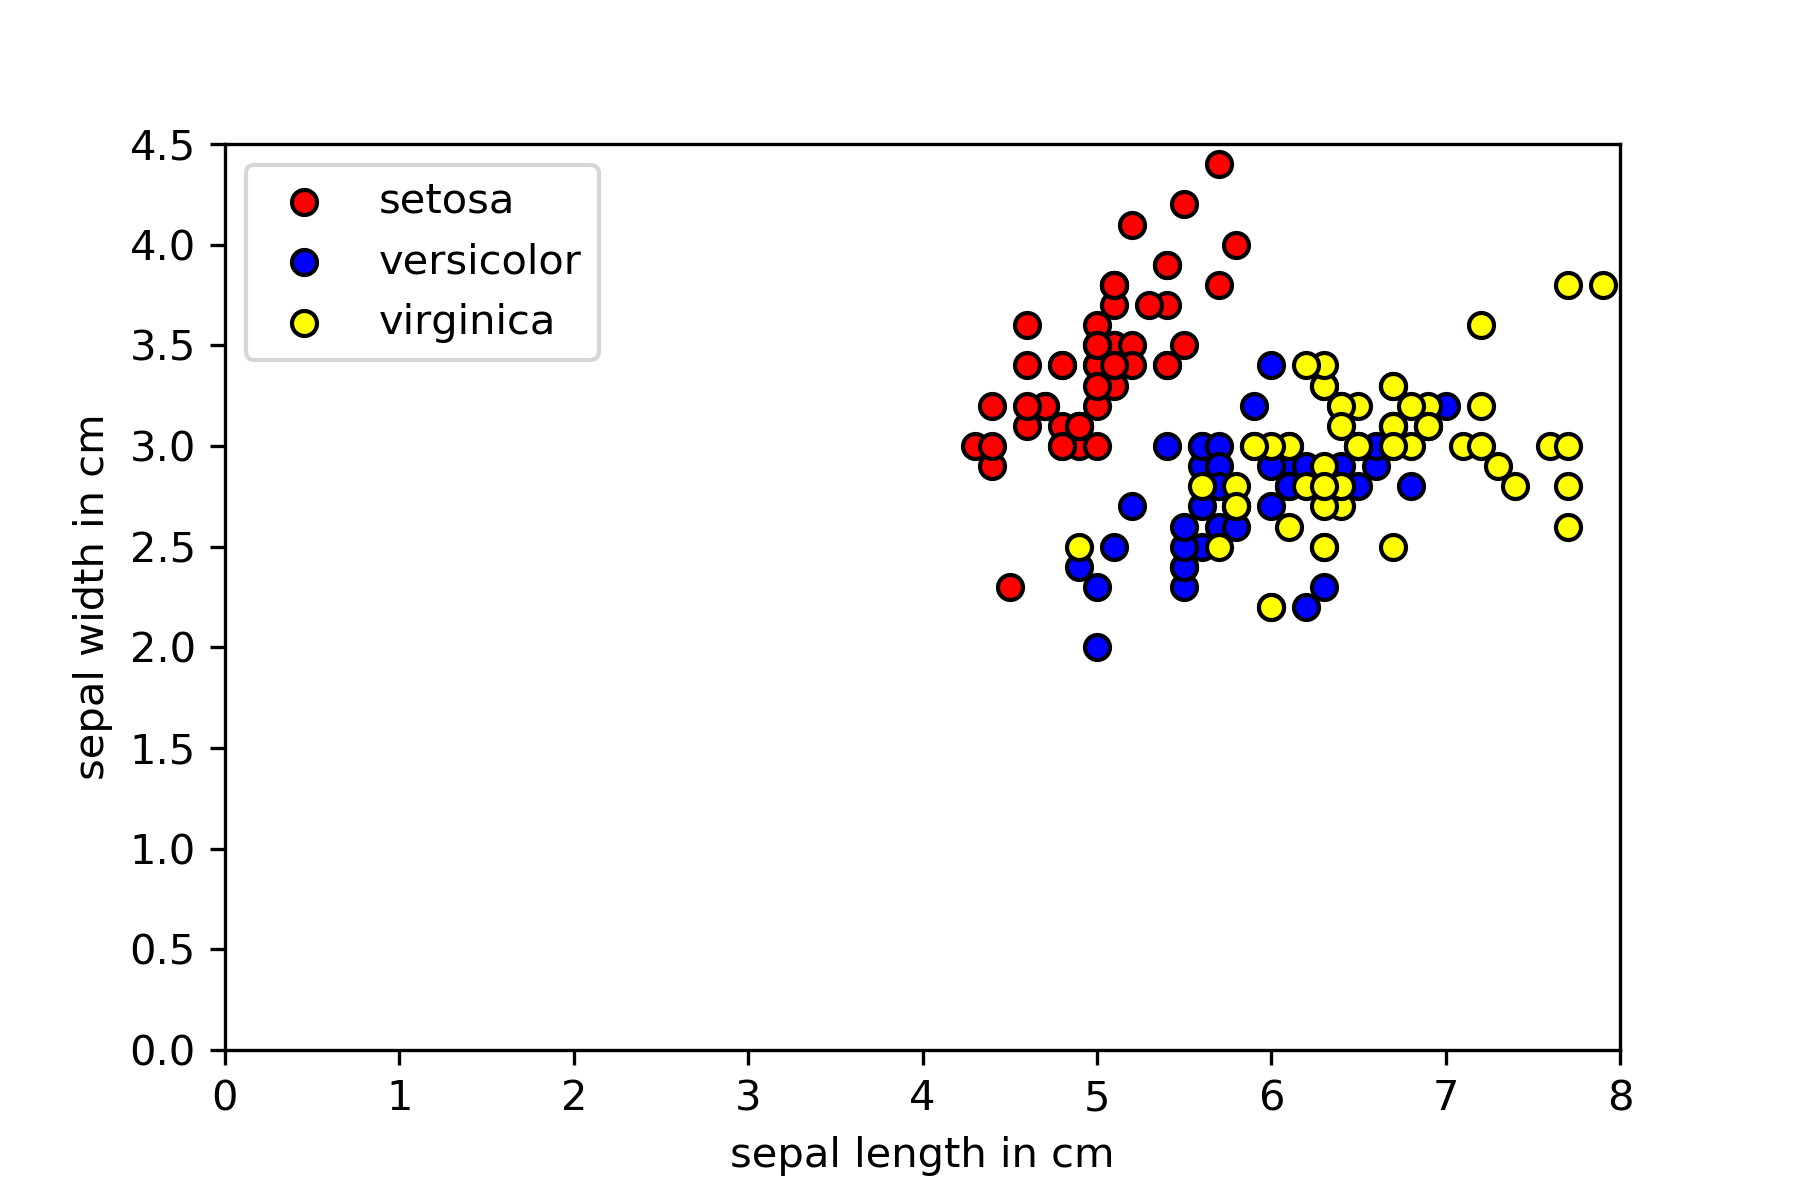
\includegraphics[width=\linewidth]{gfx/iris/iris4features}
    \caption{Data set Iris non elaborato}
    \label{fig:iris_grezzi}
\end{figure}

La prima operazione sui dati è la standardizzazione, che trasla e scala 
i punti in modo che abbiamo media nulla e deviazione standard unitaria. 
Si possono notare gli effetti nella figura \ref{fig:iris_standard}. 

\begin{figure}[h!]
    \centering
    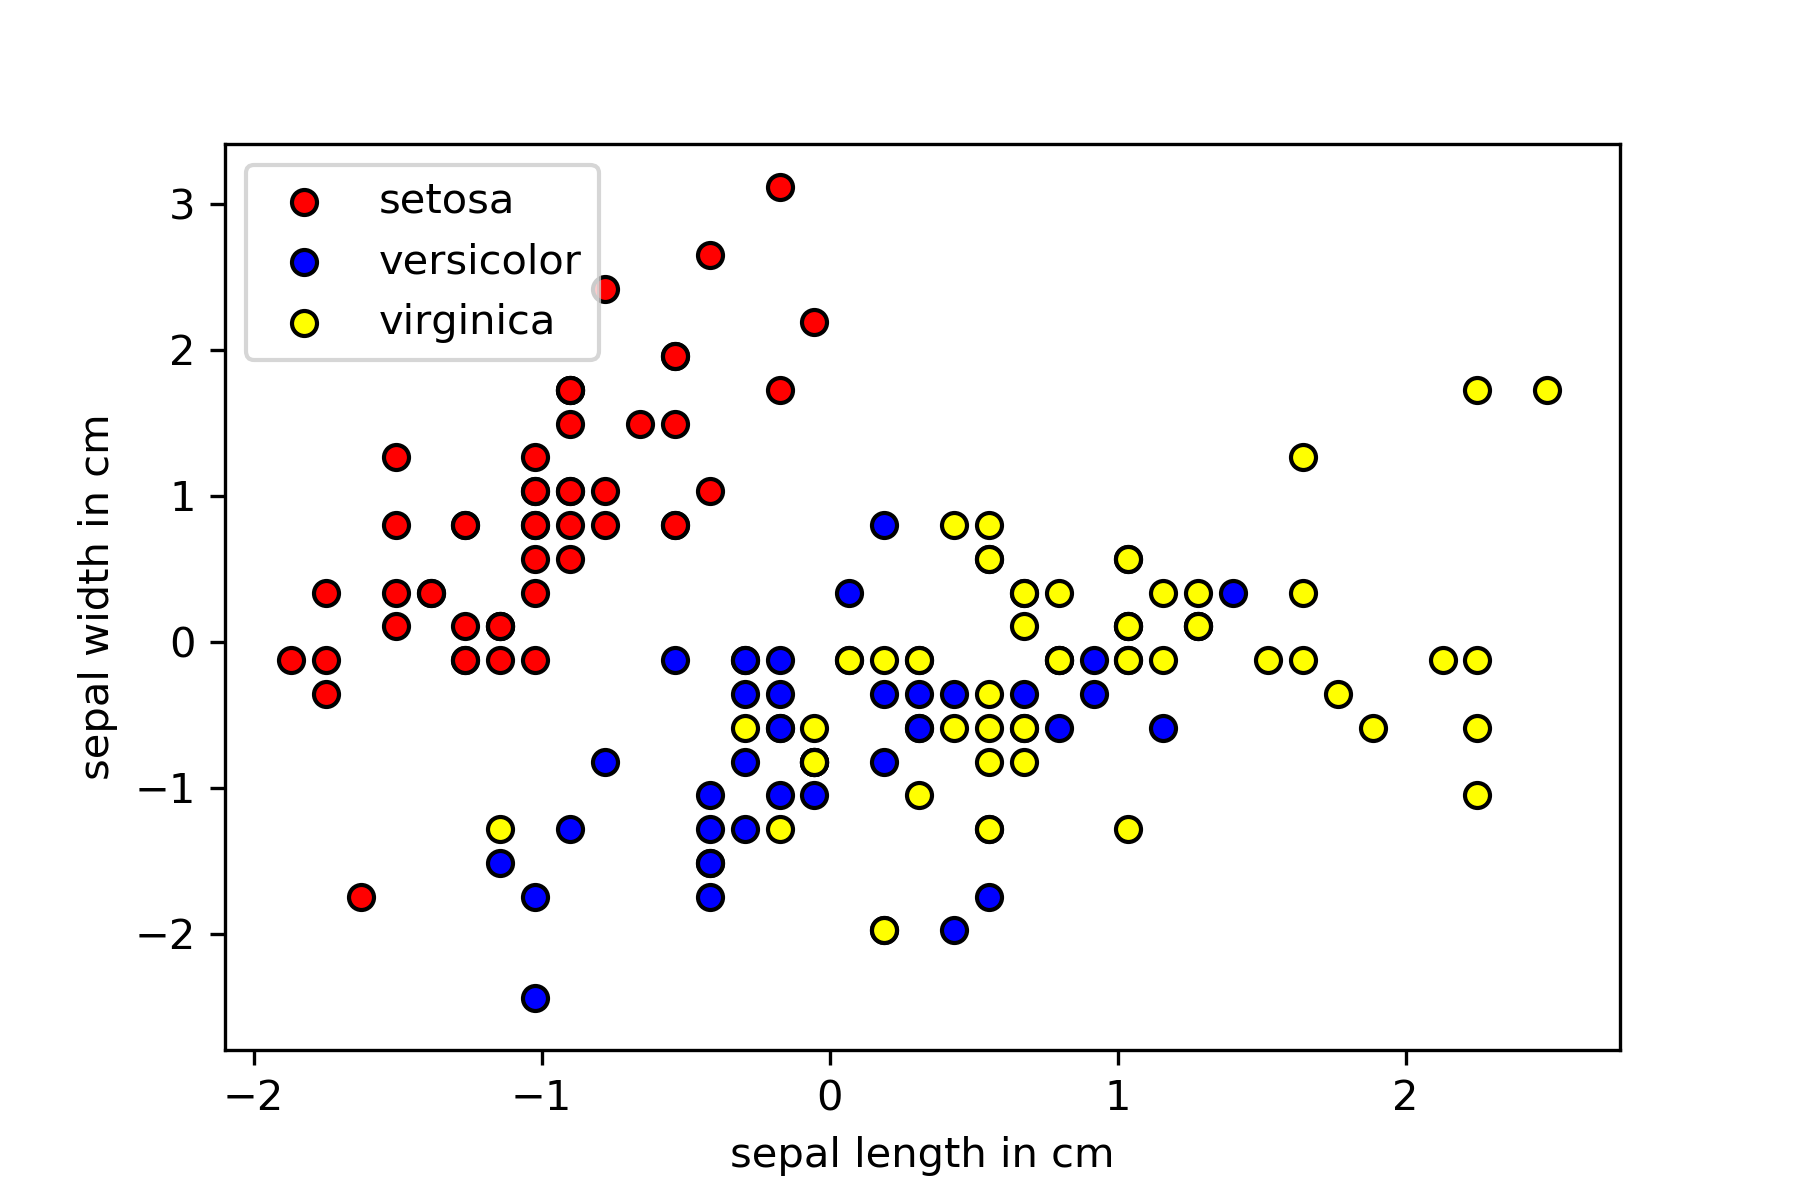
\includegraphics[width=\linewidth]{gfx/iris/irisscaled}
    \caption{Data set Iris standardizzato}
    \label{fig:iris_standard}
\end{figure}

La normalizzazione termina il processo di preparazione 
dei dati. Si può vedere l'effetto della normalizzazione su un data set 
con due o quattro caratteristiche nel riquadro \ref{fig:iris_normal}. 

\begin{figure}[htb]
    \myfloatalign
    \subfloat[2 caratteristiche]
    {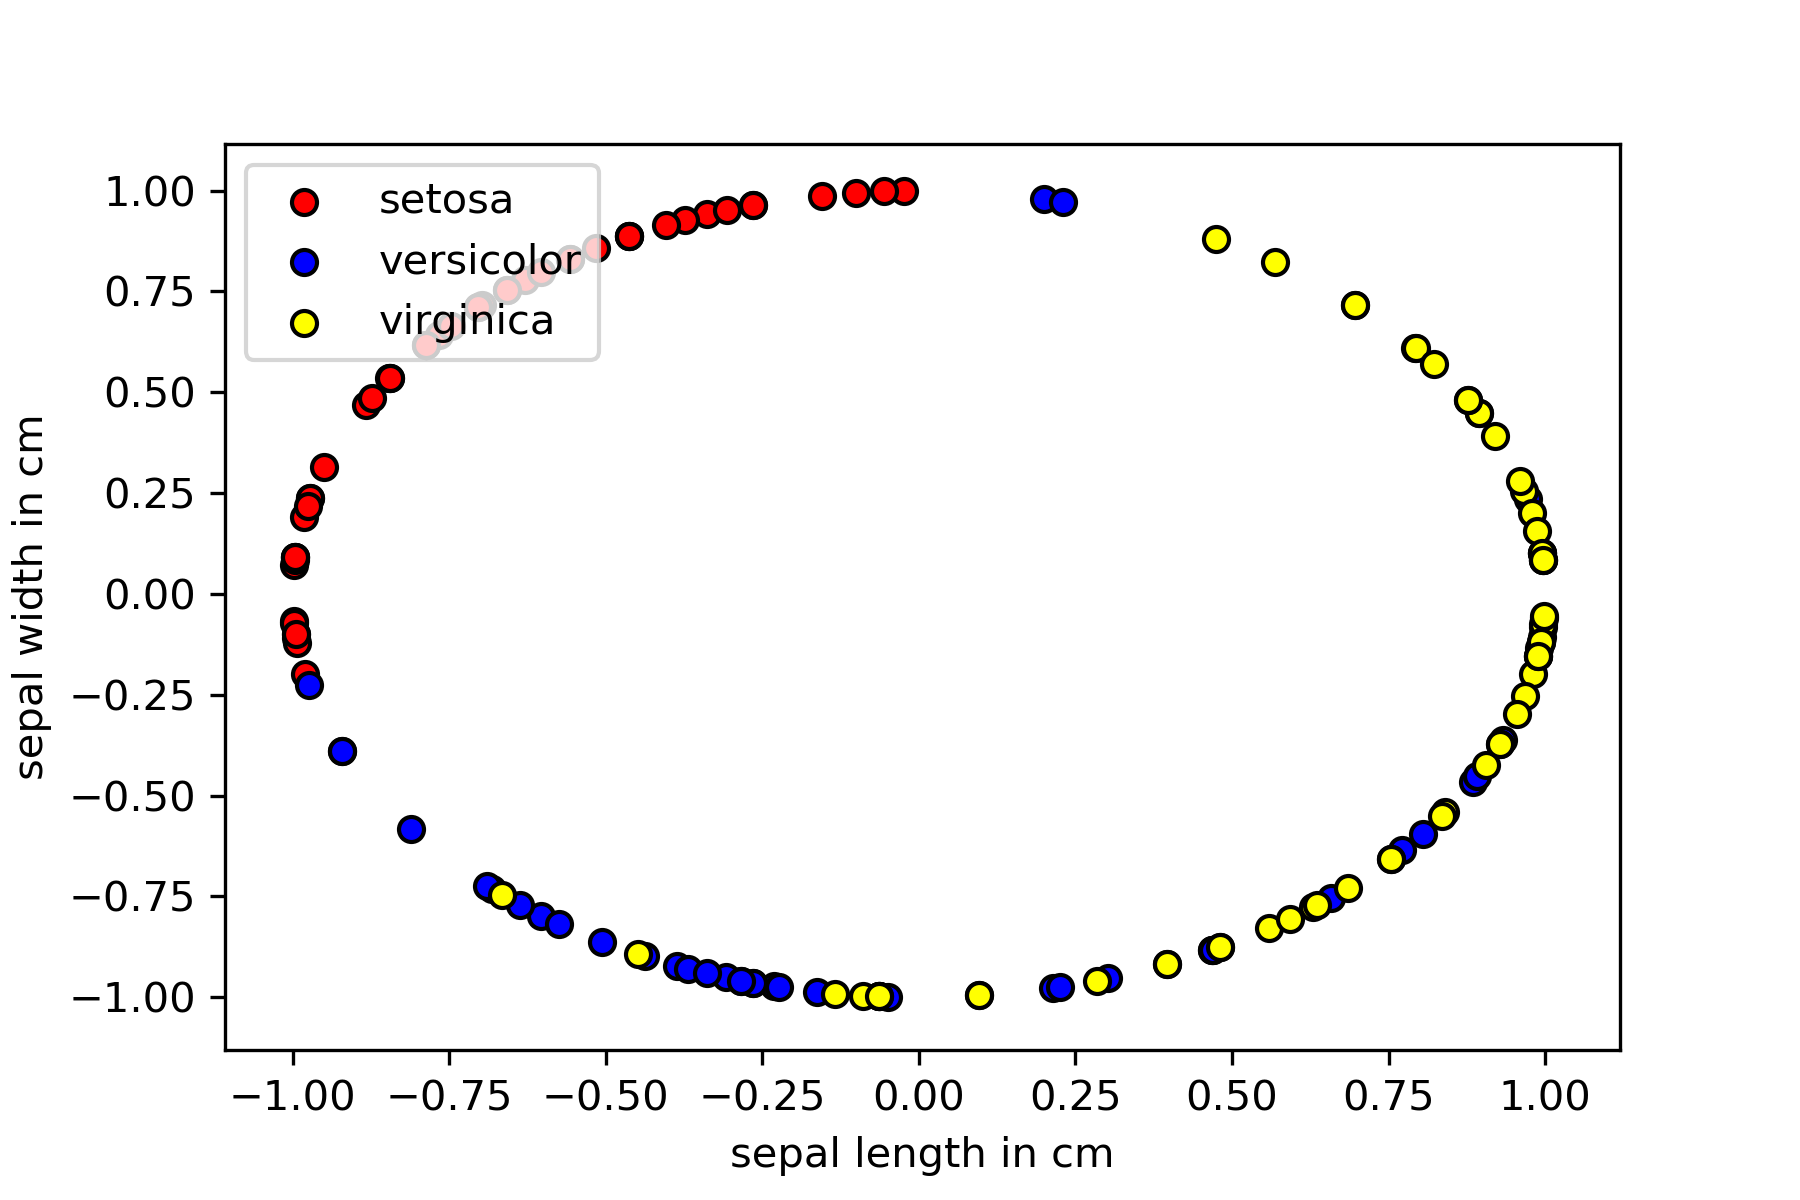
\includegraphics[width=.45\linewidth]{gfx/iris/irisnormalized}} \quad
    \subfloat[4 caratteristiche]
    {\label{fig:4caratteristiche.normalizzate}%
        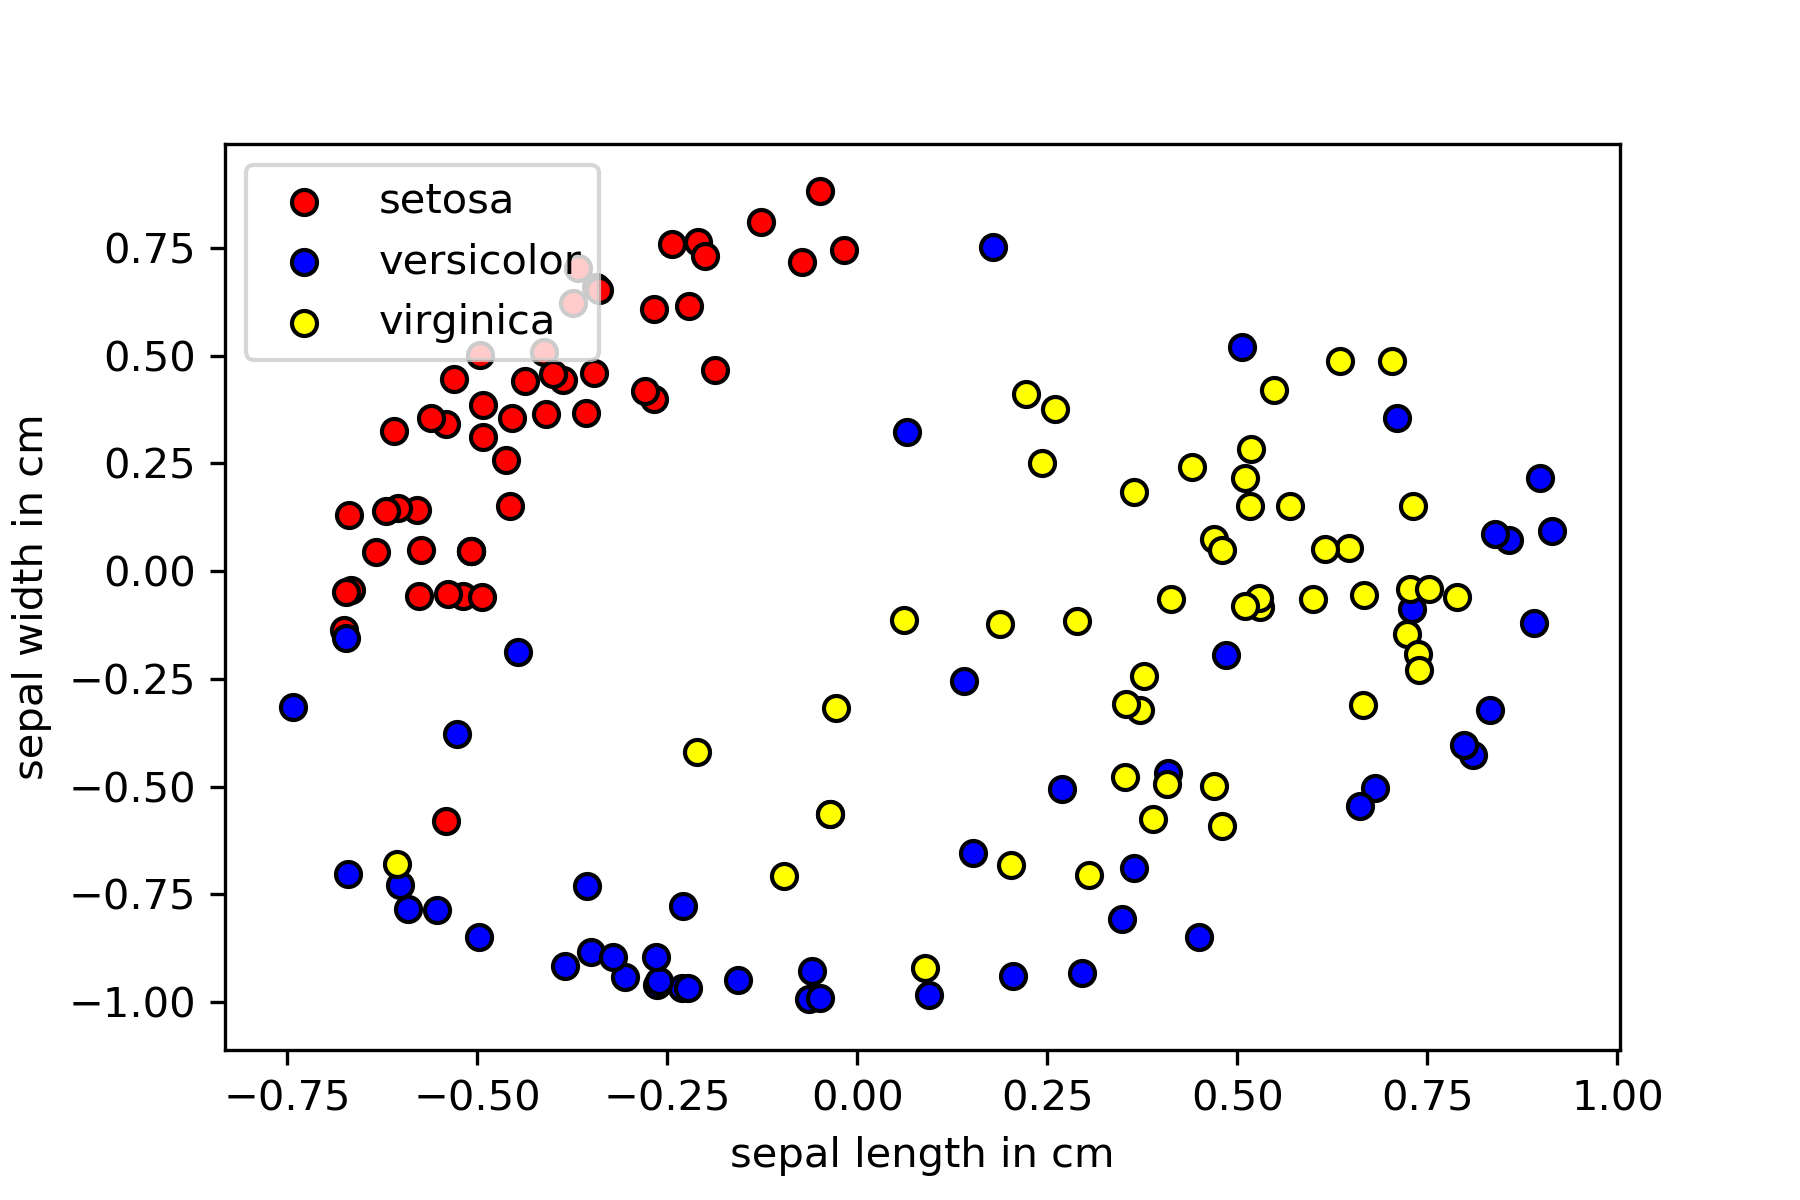
\includegraphics[width=.45\linewidth]{gfx/iris/iris4normalized}} % \\
    % \subfloat[Methodicamente o uno.]
    % {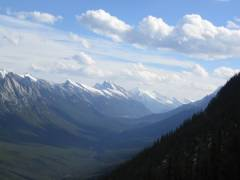
\includegraphics[width=.45\linewidth]{gfx/example_3}} \quad
    % \subfloat[Titulo debitas.]
    % {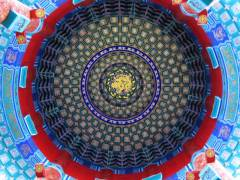
\includegraphics[width=.45\linewidth]{gfx/example_4}}
    \caption{Data set Iris normalizzato}
    \label{fig:iris_normal}
\end{figure}

% \begin{figure}[ht]
%     \centering
%     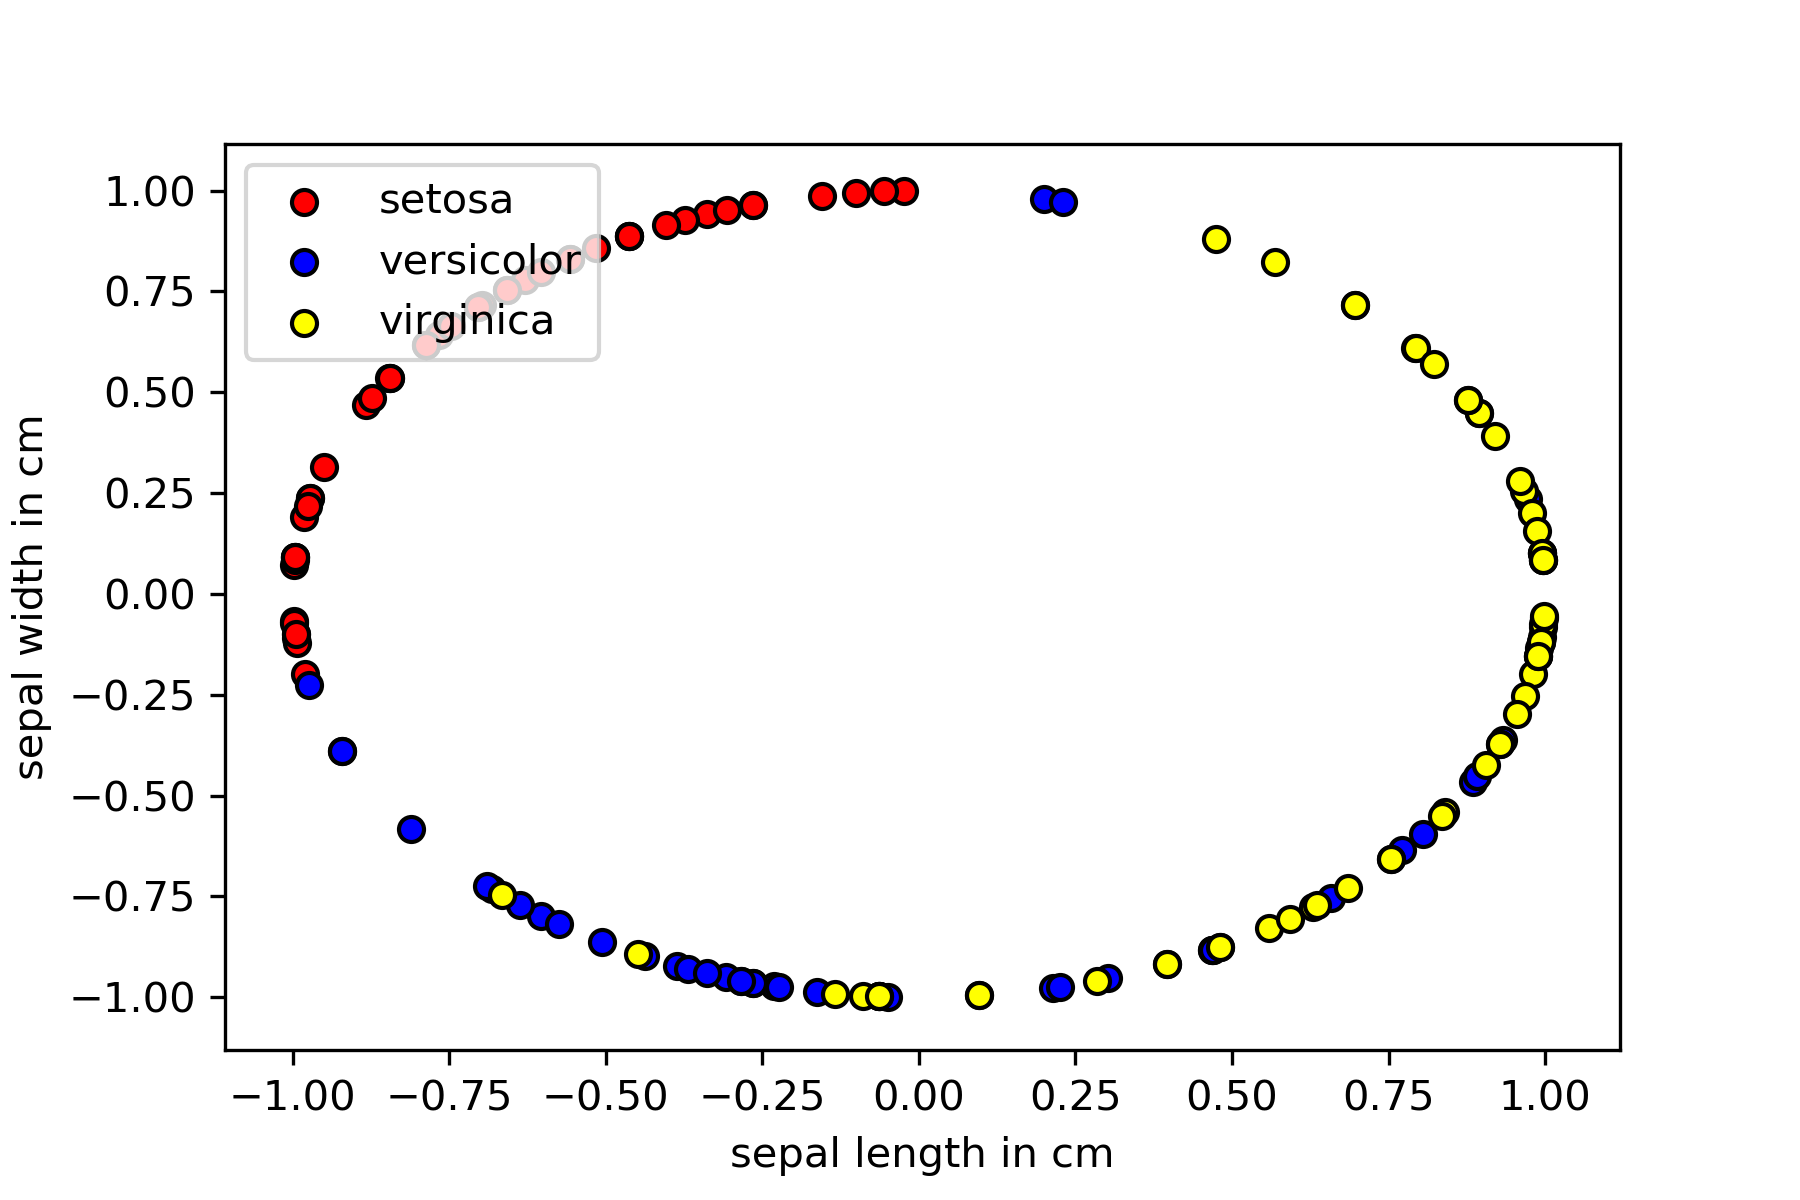
\includegraphics[width=\linewidth]{gfx/iris/irisnormalized}
%     \caption{Data set Iris normalizzato}
%     \label{fig:iris_normal}
% \end{figure}

Avendo effettuato queste operazioni, si traducono le coordinate 
di ciascun vettore nello spazio delle caratteristiche in un angolo di rotazione 
da applicare al qubit registro della \ac{QRAM}, come descritto nell'eq. \ref{eq:angolo.qram}. 

\section{Classificazione base}

% Considereremo validi per i nostri scopi solo le misure del qubit classe ottenute quando il 
% qubit ancilla è trovato nello stato $\ket{0}$. 
% Possiamo notare, tra le altre cose, che la porta $C^n R_y (\theta)$ è in 
% realtà formata da una successione di più porte di base. Mentre nei primi tempi 
% era necessario inserire manualmente i singoli elementi logici per eseguire una operazione 
% complessa, nella realizzazione attuale si è sfruttato il lavoro della comunità 
% open source di Qiskit, che ha messo a disposizione comandi veloci per aggiungere 
% facilmente porte multi controllate. 

Per dare un esempio di classificazione binaria tra le classi setosa e 
versicolor si sono usate le prime due caratteristiche e si sono posti 
a confronto il vettore 29 (setosa) e 57 (versicolor) in input con i 
due vettori di training 34 (setosa) e 86 (versicolor). 
La classe setosa è stata collegata allo stato $\ket{c=0}$, la classe 
versicolor allo stato $\ket{c=1}$.
I risultati ottenuti da una simulazione su computer portatile sono 
visibili in figura \ref{fig:simulazione_circuito}. 
Nella didascalia sono scritti i conteggi totali corrispondenti ad un determinato 
esito di misura sui due qubit ancilla e classe. 
La cifra sulla destra contiene la misura del qubit ancilla, quella sulla 
sinistra del qubit classe. 
L'istogramma riporta la normalizzazione unitaria dei risultati, che approssima 
la distribuzione di probabilità per numeri grandi di esecuzioni dell'algoritmo. 
Si userà preferibilmente un numero di esecuzioni (shot) pari al massimo permesso 
dai computer quantistici dell'IBM, ovvero 8192. 

% Per dare un esempio di risultato di classificazione usando solo le prime due caratteristiche 
% del data set e gli elementi appartenenti alle classi setosa e versicolor. 
% Si scelgono come vettori di training un elemento per ciascuna classe, nel nostro caso 
% il vettore 34 ed il vettore 86 dal data set, rispettivamente setosa e versicolor. 
% Si assegna alla classe setosa lo stato $\ket{0}$ del qubit classe ed alla classe 
% versicolor lo stato $\ket{1}$. 
% Si sottopongono poi a classificazione, in due esperimenti separati, due vettori sconosciuti: 
% il vettore 29 (setosa) ed il vettore 57 (versicolor). 

% Il primo passo è simulare l'esperimento sul computer in uso, dato che il problema in esame
% è facilmente eseguibile su un comune portatile. I risultati non filtrati per i due esperimenti 
% sono visibili nel riquadro \ref{fig:simulazione_circuito}. Nella didascalia sono scritti i conteggi corrispondenti ad un 
% determinato esito di misura sui due qubit ancilla e classe. La cifra sulla destra contiene la 
% misura del qubit ancilla, quella sulla sinistra del qubit classe. Tali valori, normalizzati ad uno, 
% sono rappresentati in un istogramma, che approssima la distribuzione di probabilità degli esiti di 
% misura per grandi numeri di esecuzioni dell'algoritmo. Per questo motivo si userà preferibilmente 
% un numero di esecuzioni pari al massimo permesso sui computer quantistici dell'IBM, ovvero 8192. 

% \begin{figure}[h!]
%     \myfloatalign
%     \hspace{-1cm}
%     \subfloat[Iris setosa]
%     {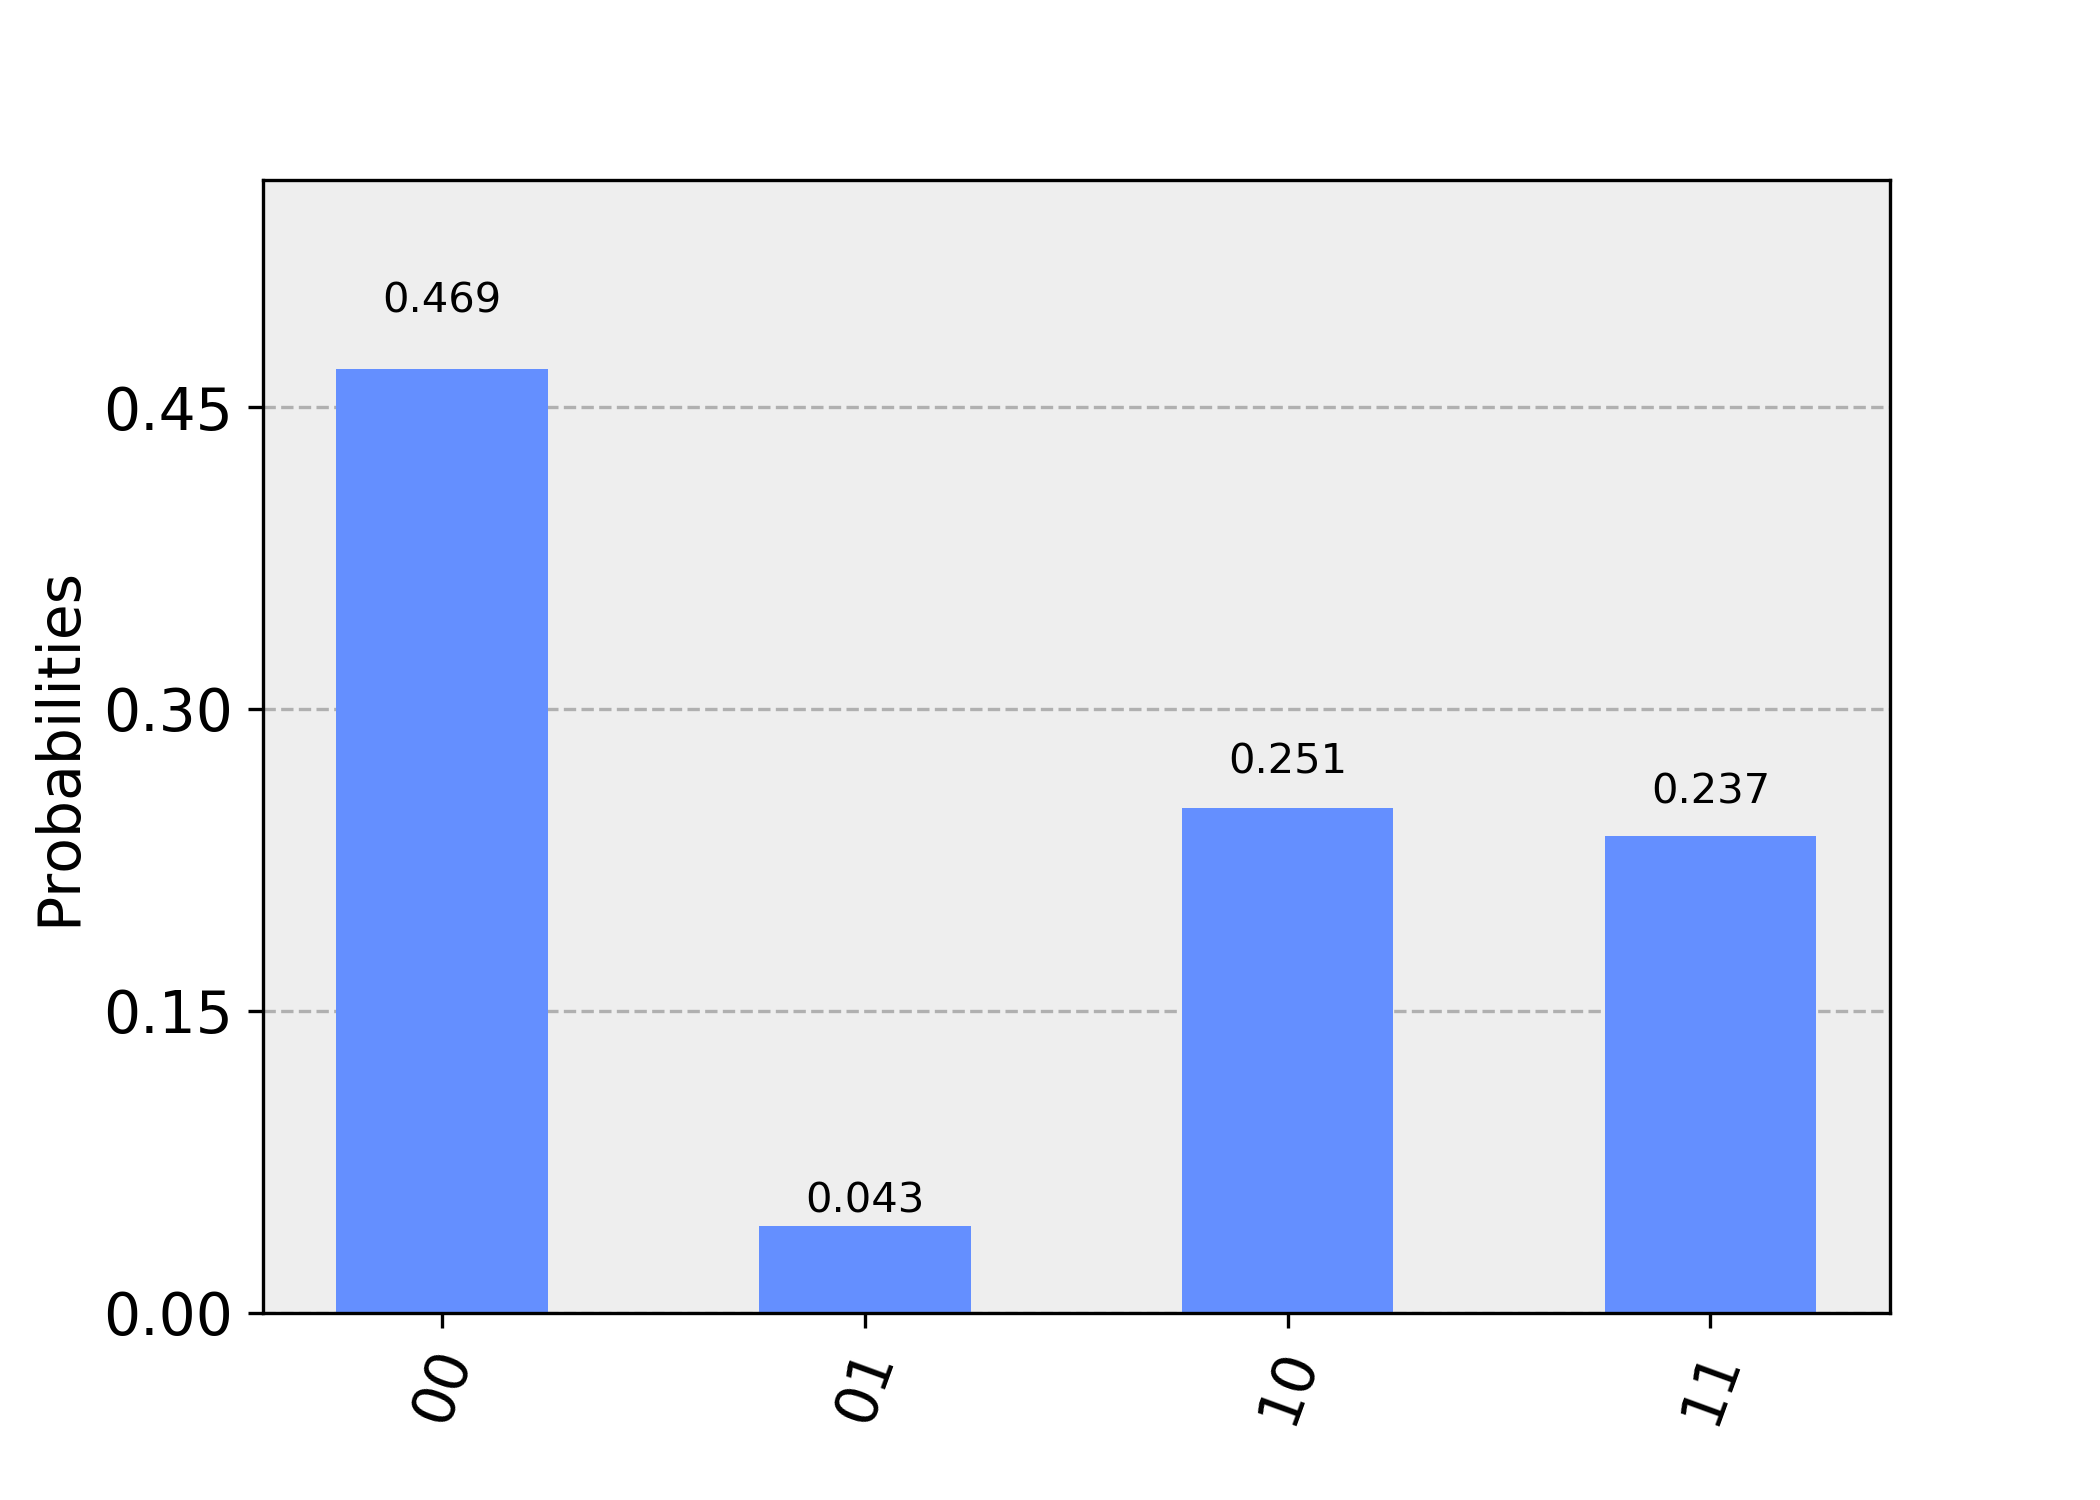
\includegraphics[width=.75\linewidth]{gfx/misura_setosa}}
%     \subfloat[Iris versicolor]
%     {%\label{fig:example-b}%
%         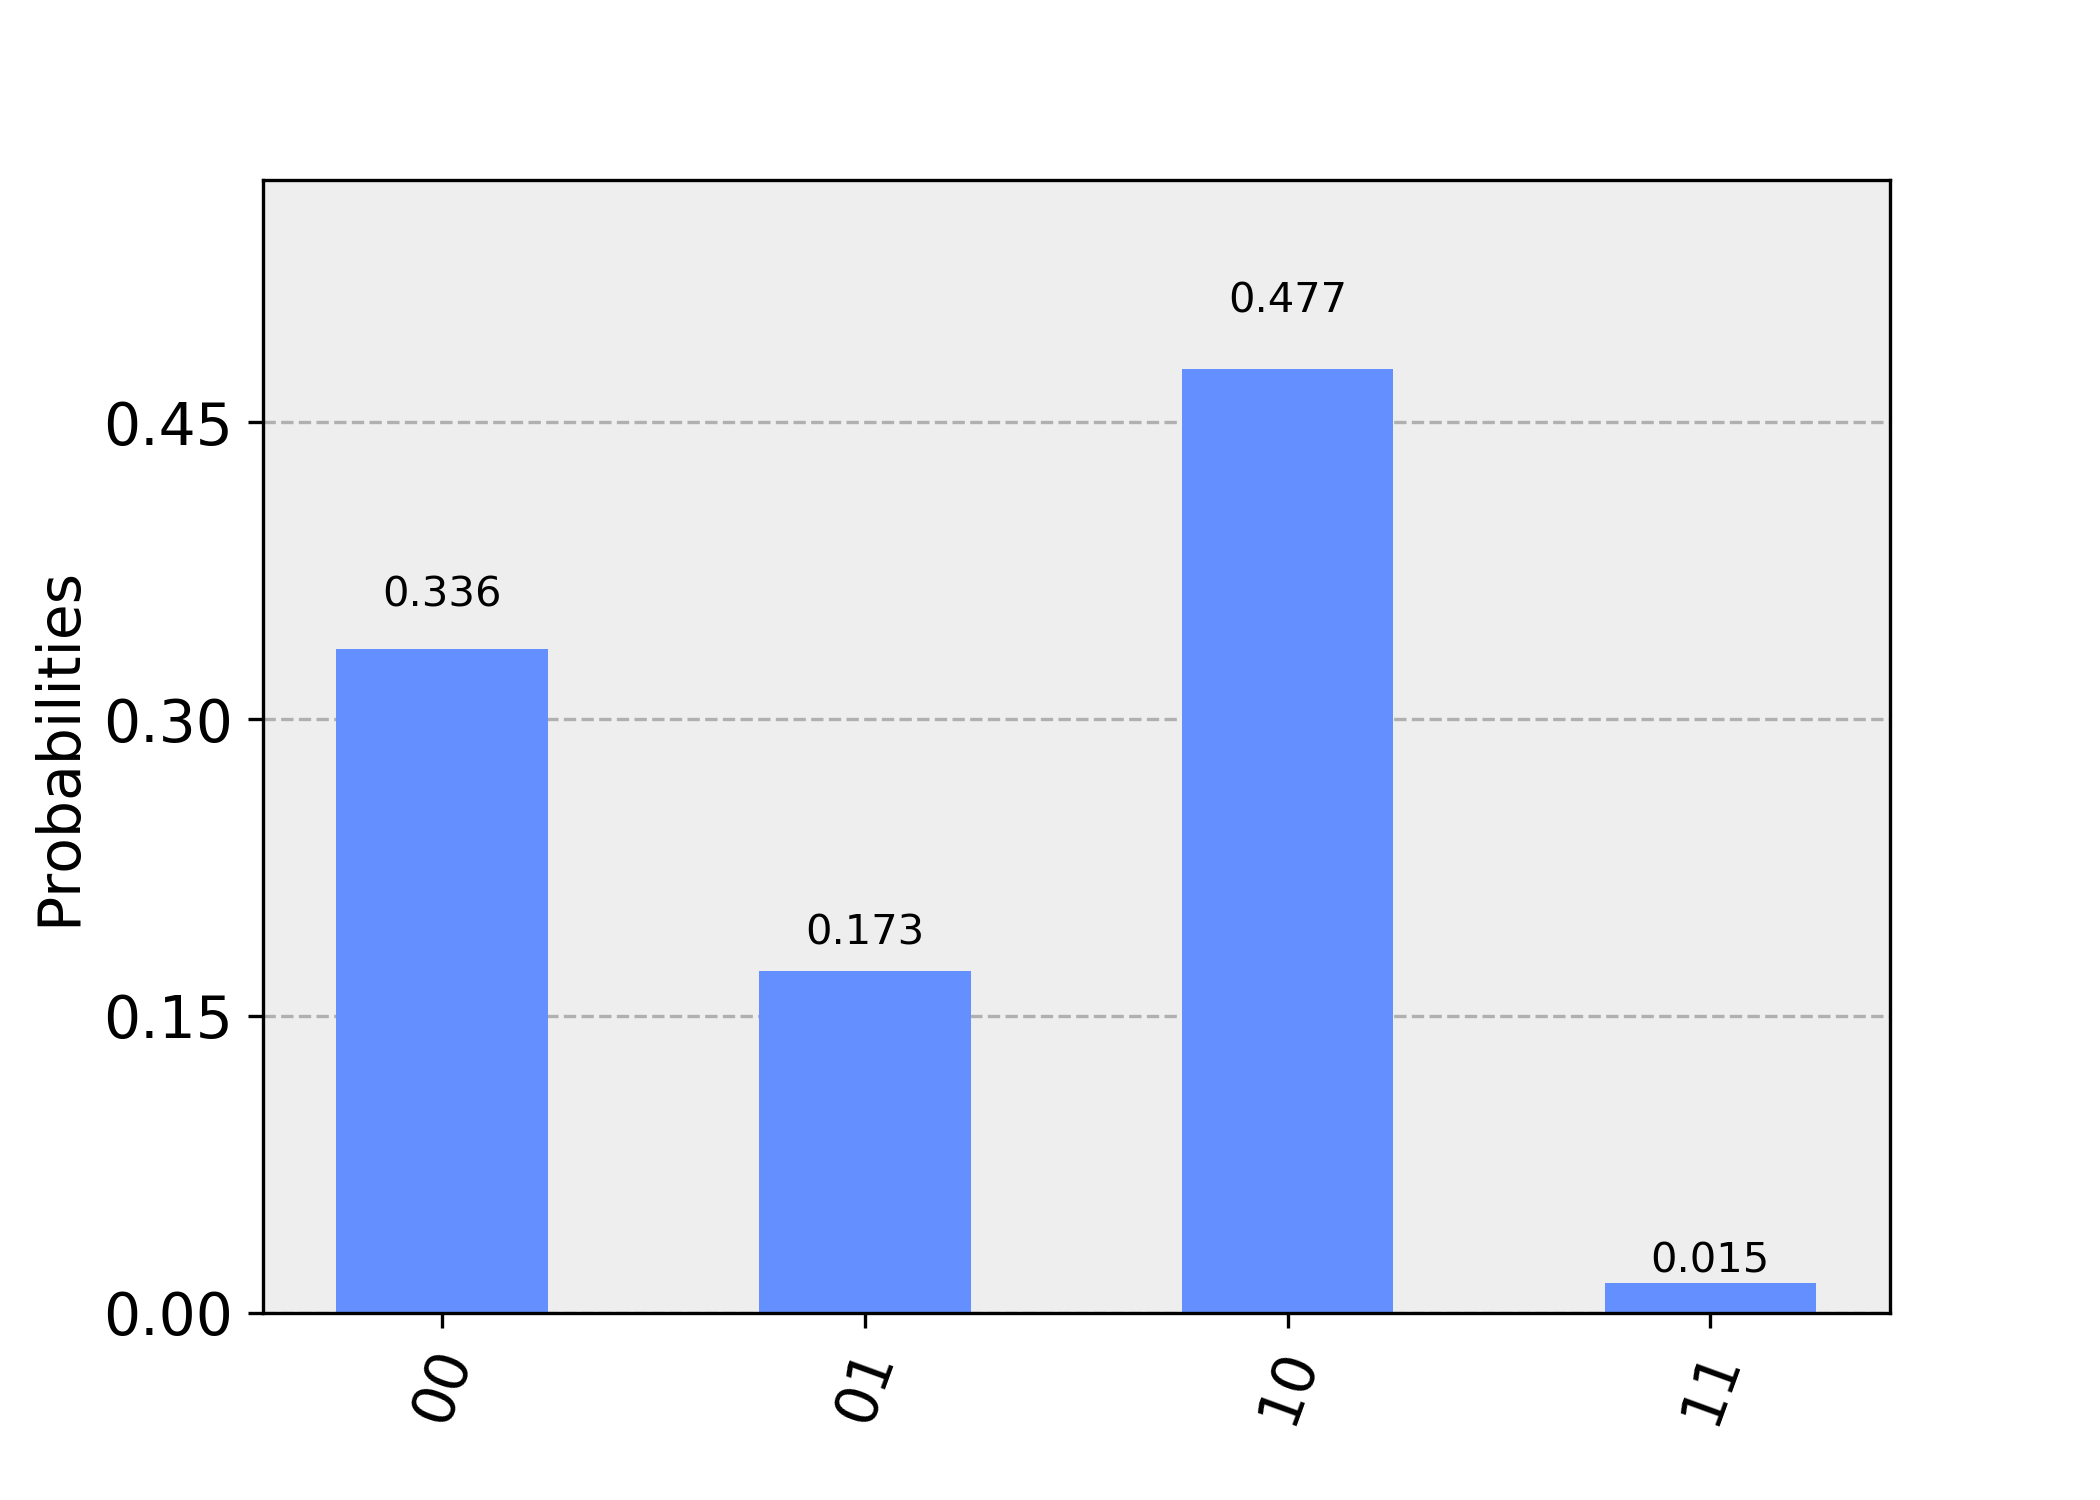
\includegraphics[width=.75\linewidth]{gfx/misura_versicolor}} % \\
%     % \subfloat[Iris setosa]
%     % {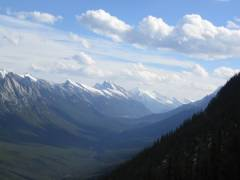
\includegraphics[width=.45\linewidth]{gfx/example_3}} \quad
%     % \subfloat[Titulo debitas.]
%     % {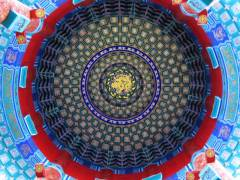
\includegraphics[width=.45\linewidth]{gfx/example_4}}
%     \caption[Simulazione del circuito]%
%     {Simulazione del circuito. \par \small 
%     I conteggi totali sono: \\
%     per setosa \{'00': 3843, '10': 2056, '01': 352, '11': 1941\}; \\
%     per versicolor \{'00': 2749, '10': 3908, '01': 1414, '11': 121\}.}%
%     \label{fig:simulazione_circuito}
% \end{figure}

\begin{figure}[h!]
    \myfloatalign
    \subfloat[Iris setosa] {
        \label{fig:misura_setosa}
        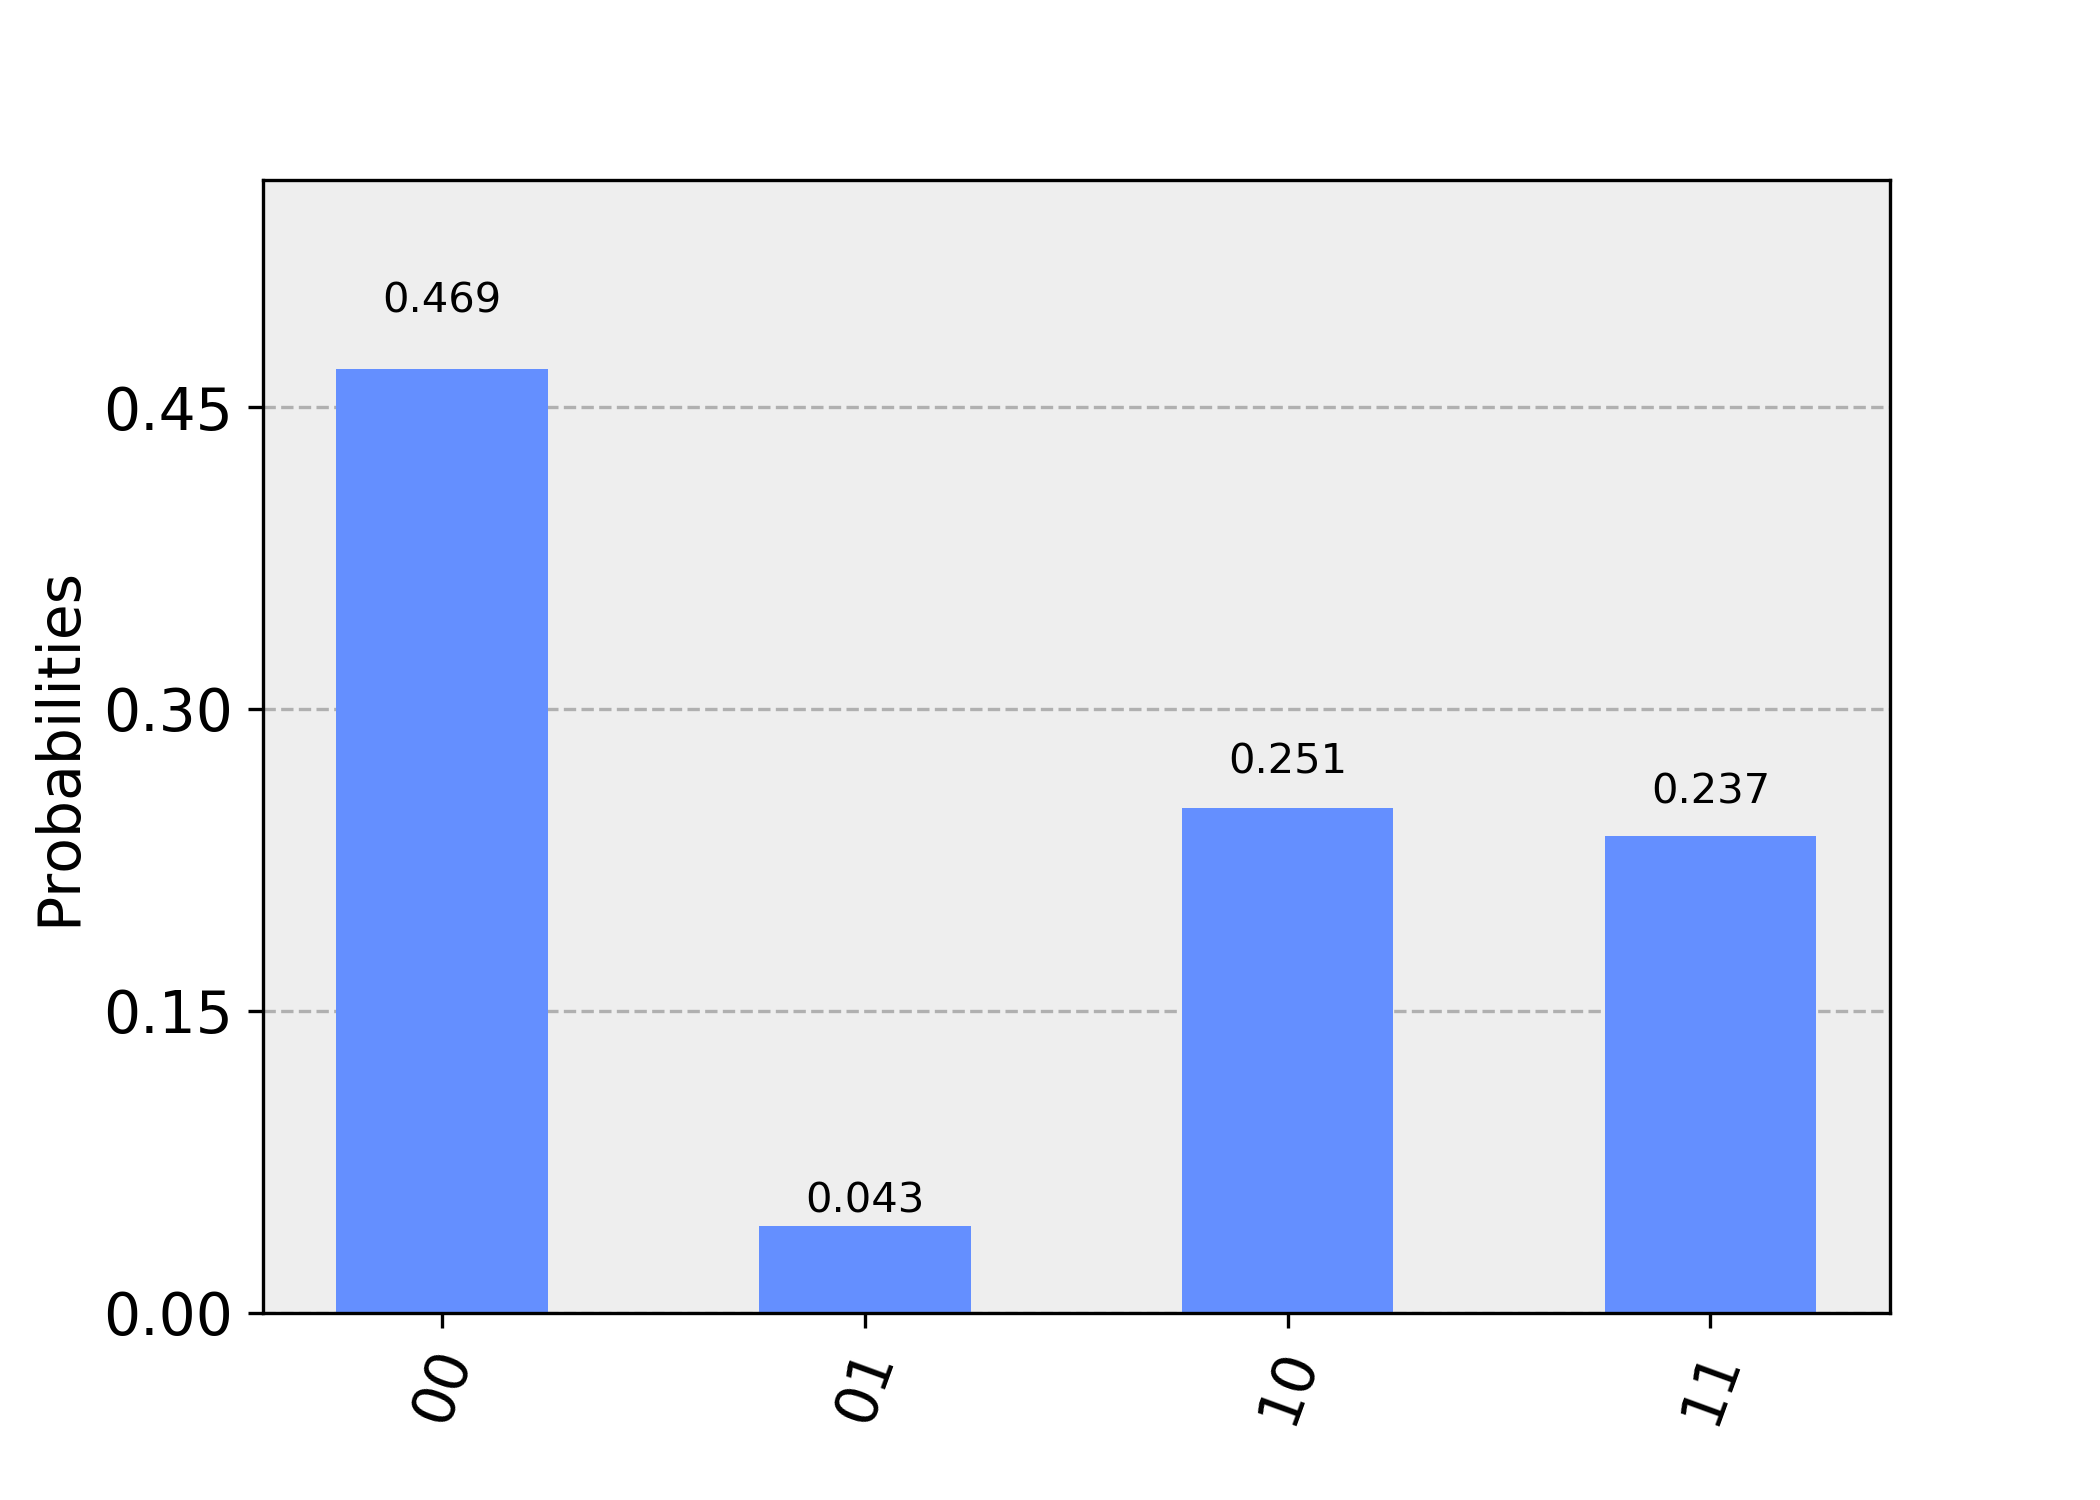
\includegraphics[width=\linewidth]{gfx/misura_setosa}
    } \\
    \subfloat[Iris versicolor] {
        \label{fig:misura_versicolor}
        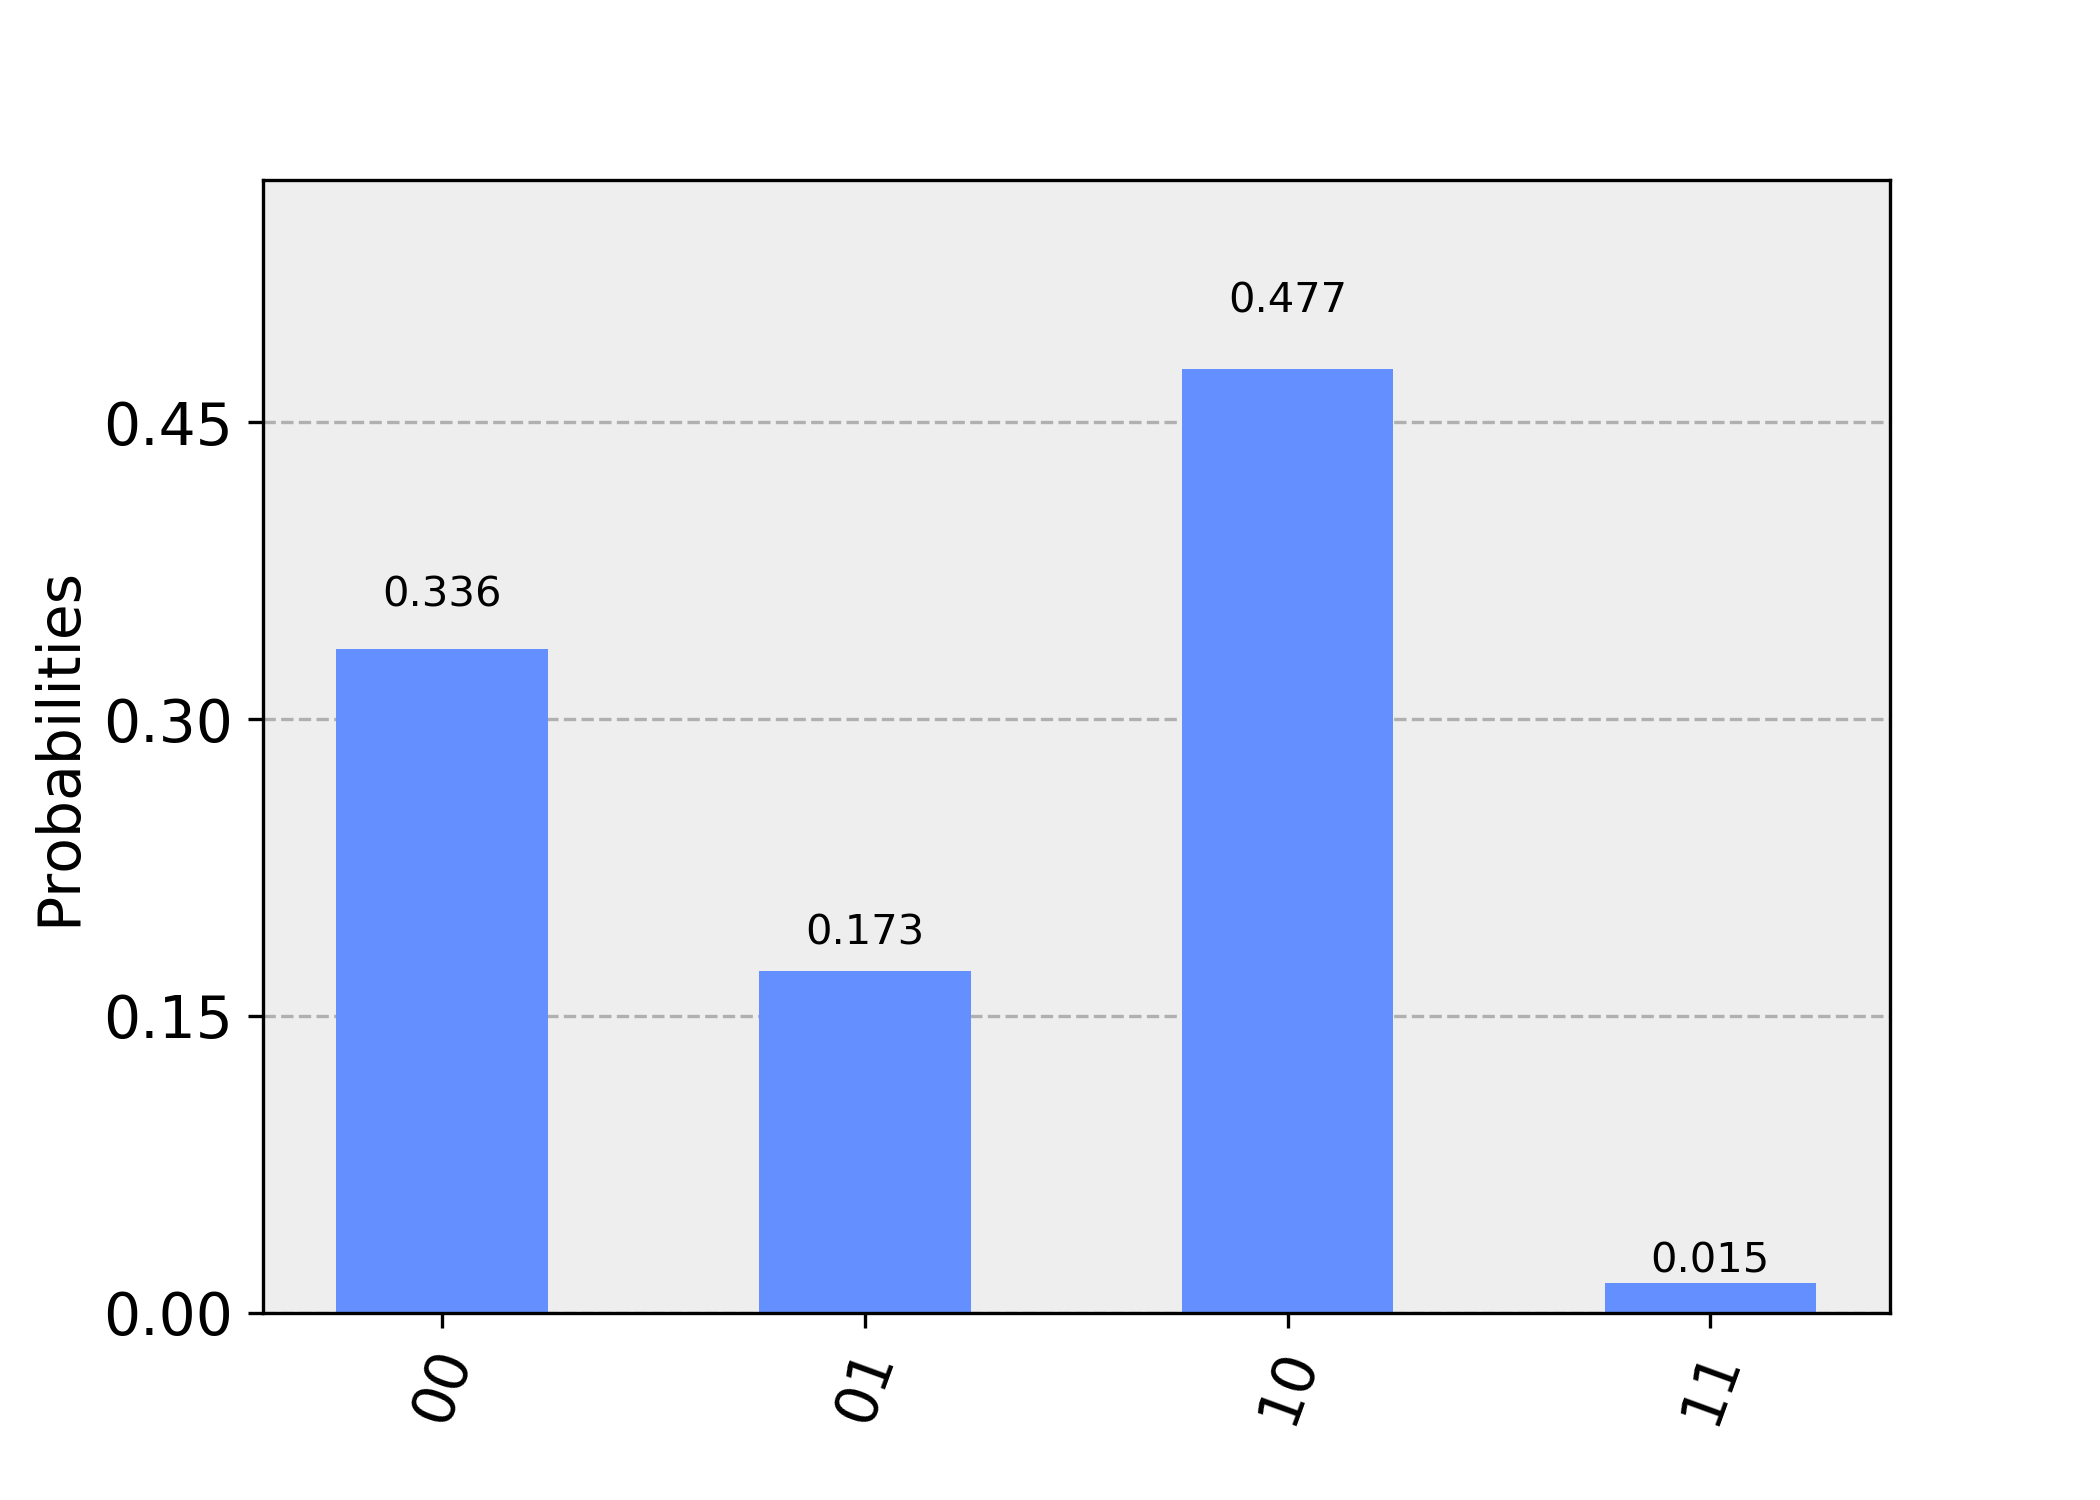
\includegraphics[width=\linewidth]{gfx/misura_versicolor}
    }
    \caption[Simulazione del circuito]%
    {Simulazione del circuito. \par \small 
    I conteggi totali sono: \\
    per setosa \{'00': 3843, '10': 2056, '01': 352, '11': 1941\}; \\
    per versicolor \{'00': 2749, '10': 3908, '01': 1414, '11': 121\}.}
    \label{fig:simulazione_circuito}
\end{figure}

Selezionando i risultati laddove il bit di destra è 0, abbiamo praticamente effettuato 
la misura condizionale necessaria al funzionamento dell'algoritmo. 
Nel riquadro \ref{fig:simulazione_filtrati} sono presentati 
i risultati filtrati dove il bit ancilla è 0. 

\begin{figure}[h!]
    \myfloatalign
    \subfloat[Iris setosa]{
        \label{fig:misura_setosa_filtrata}
        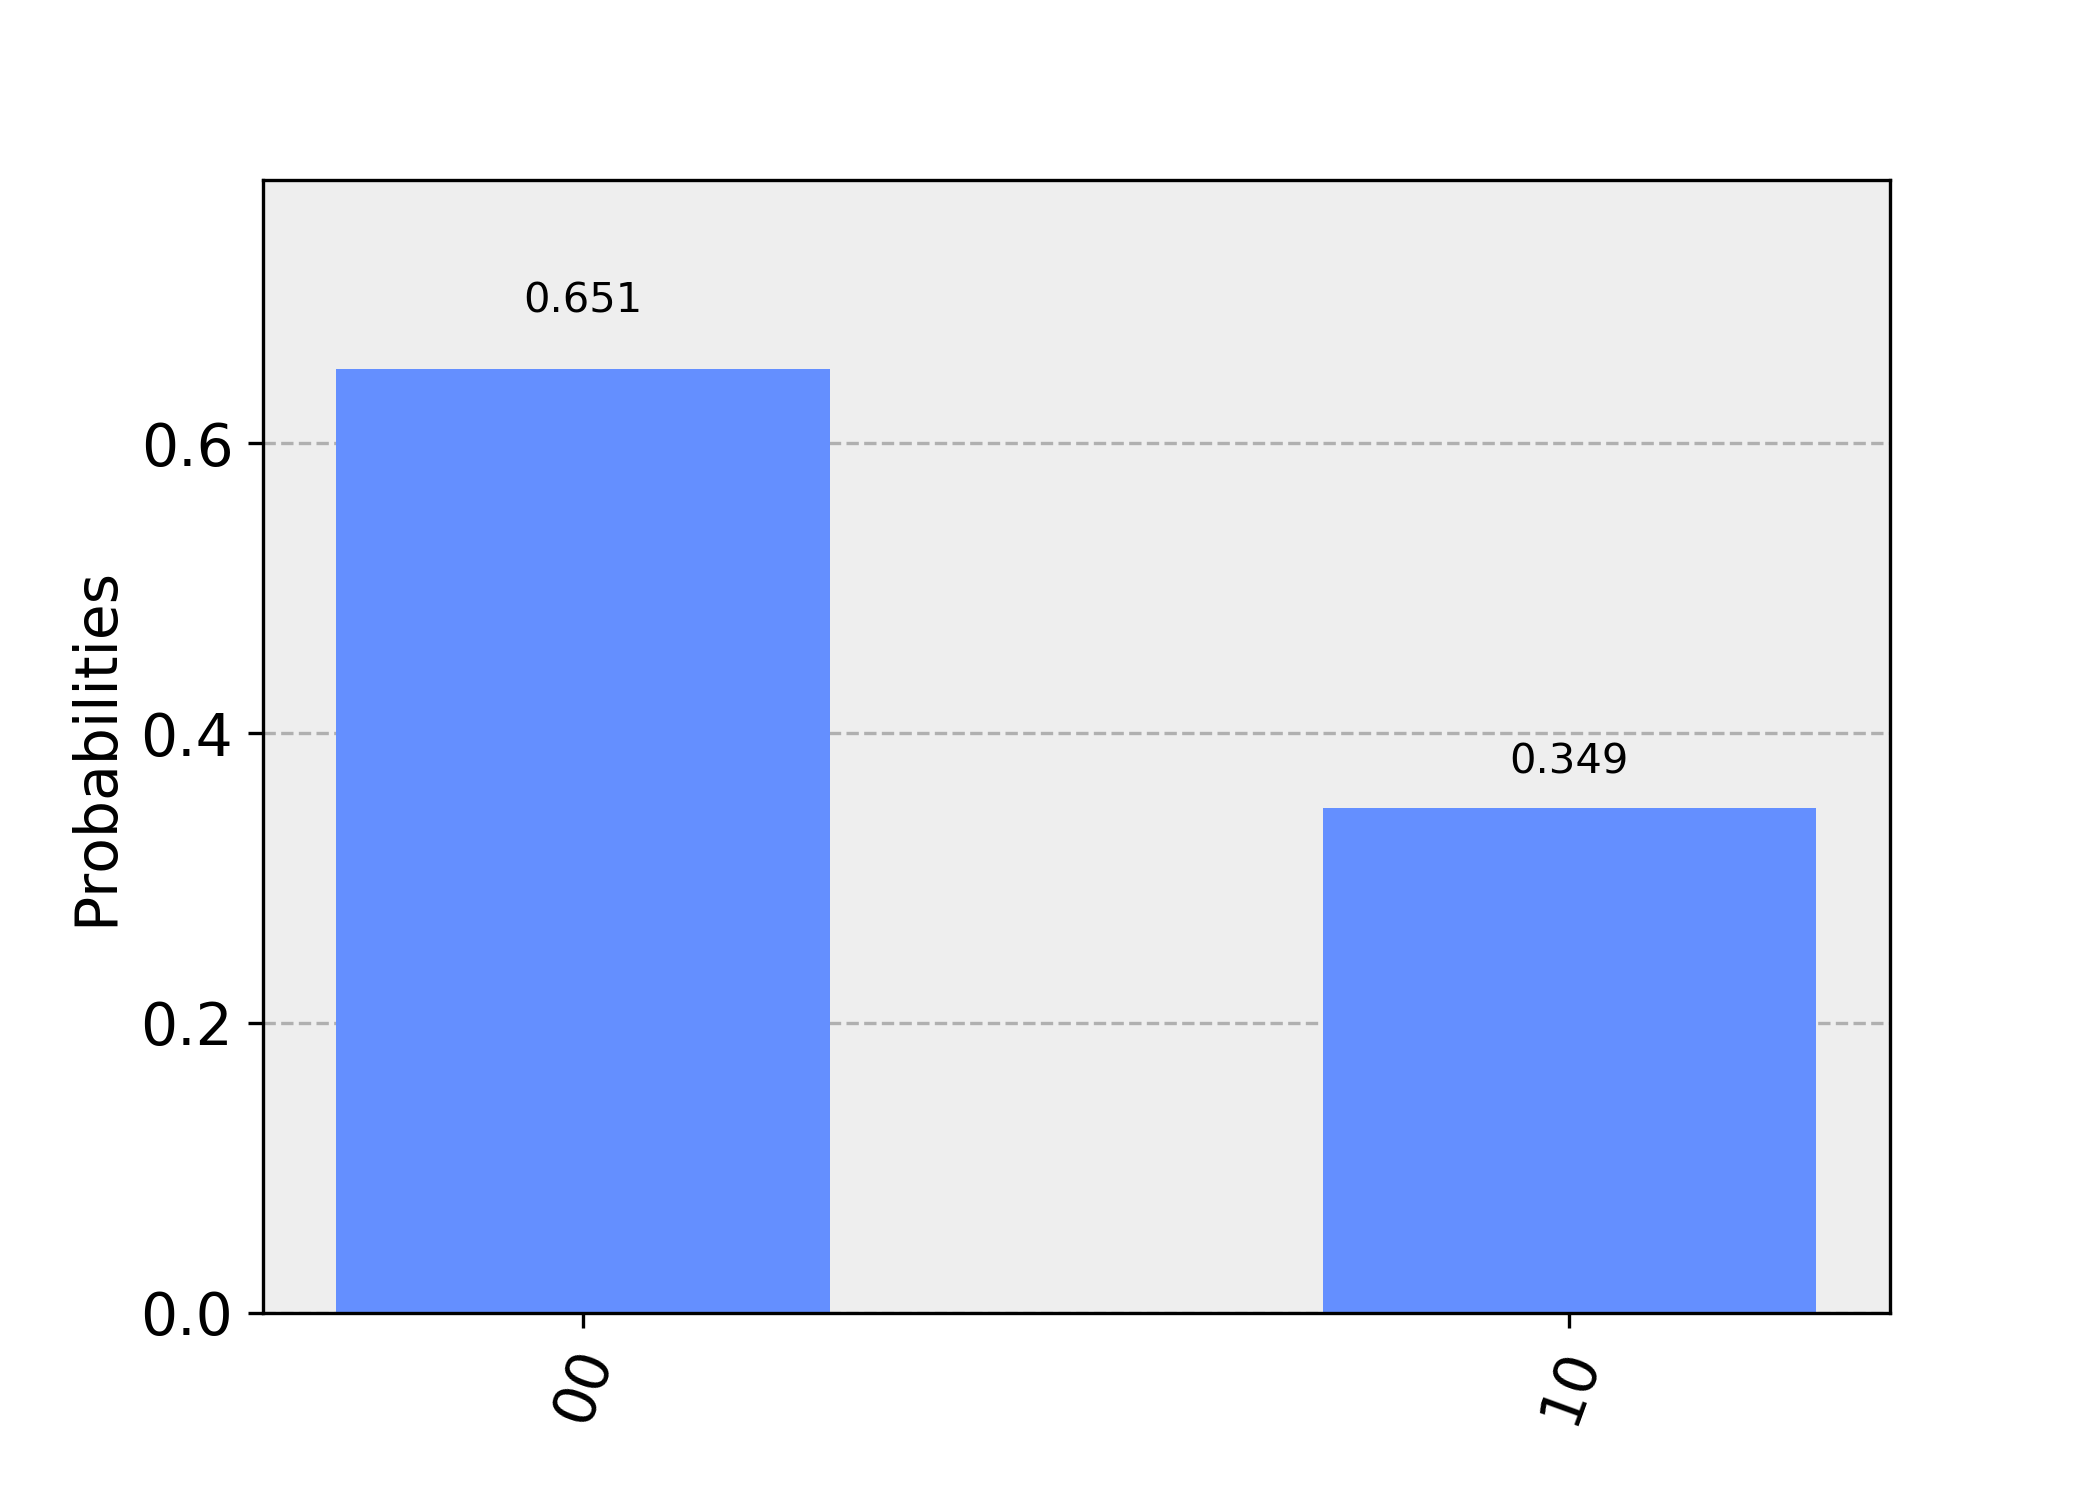
\includegraphics[width=\linewidth]{gfx/misura_setosa_filtrata}
    } \\
    \subfloat[Iris versicolor]{
        \label{fig:misura_versicolor_filtrata}
        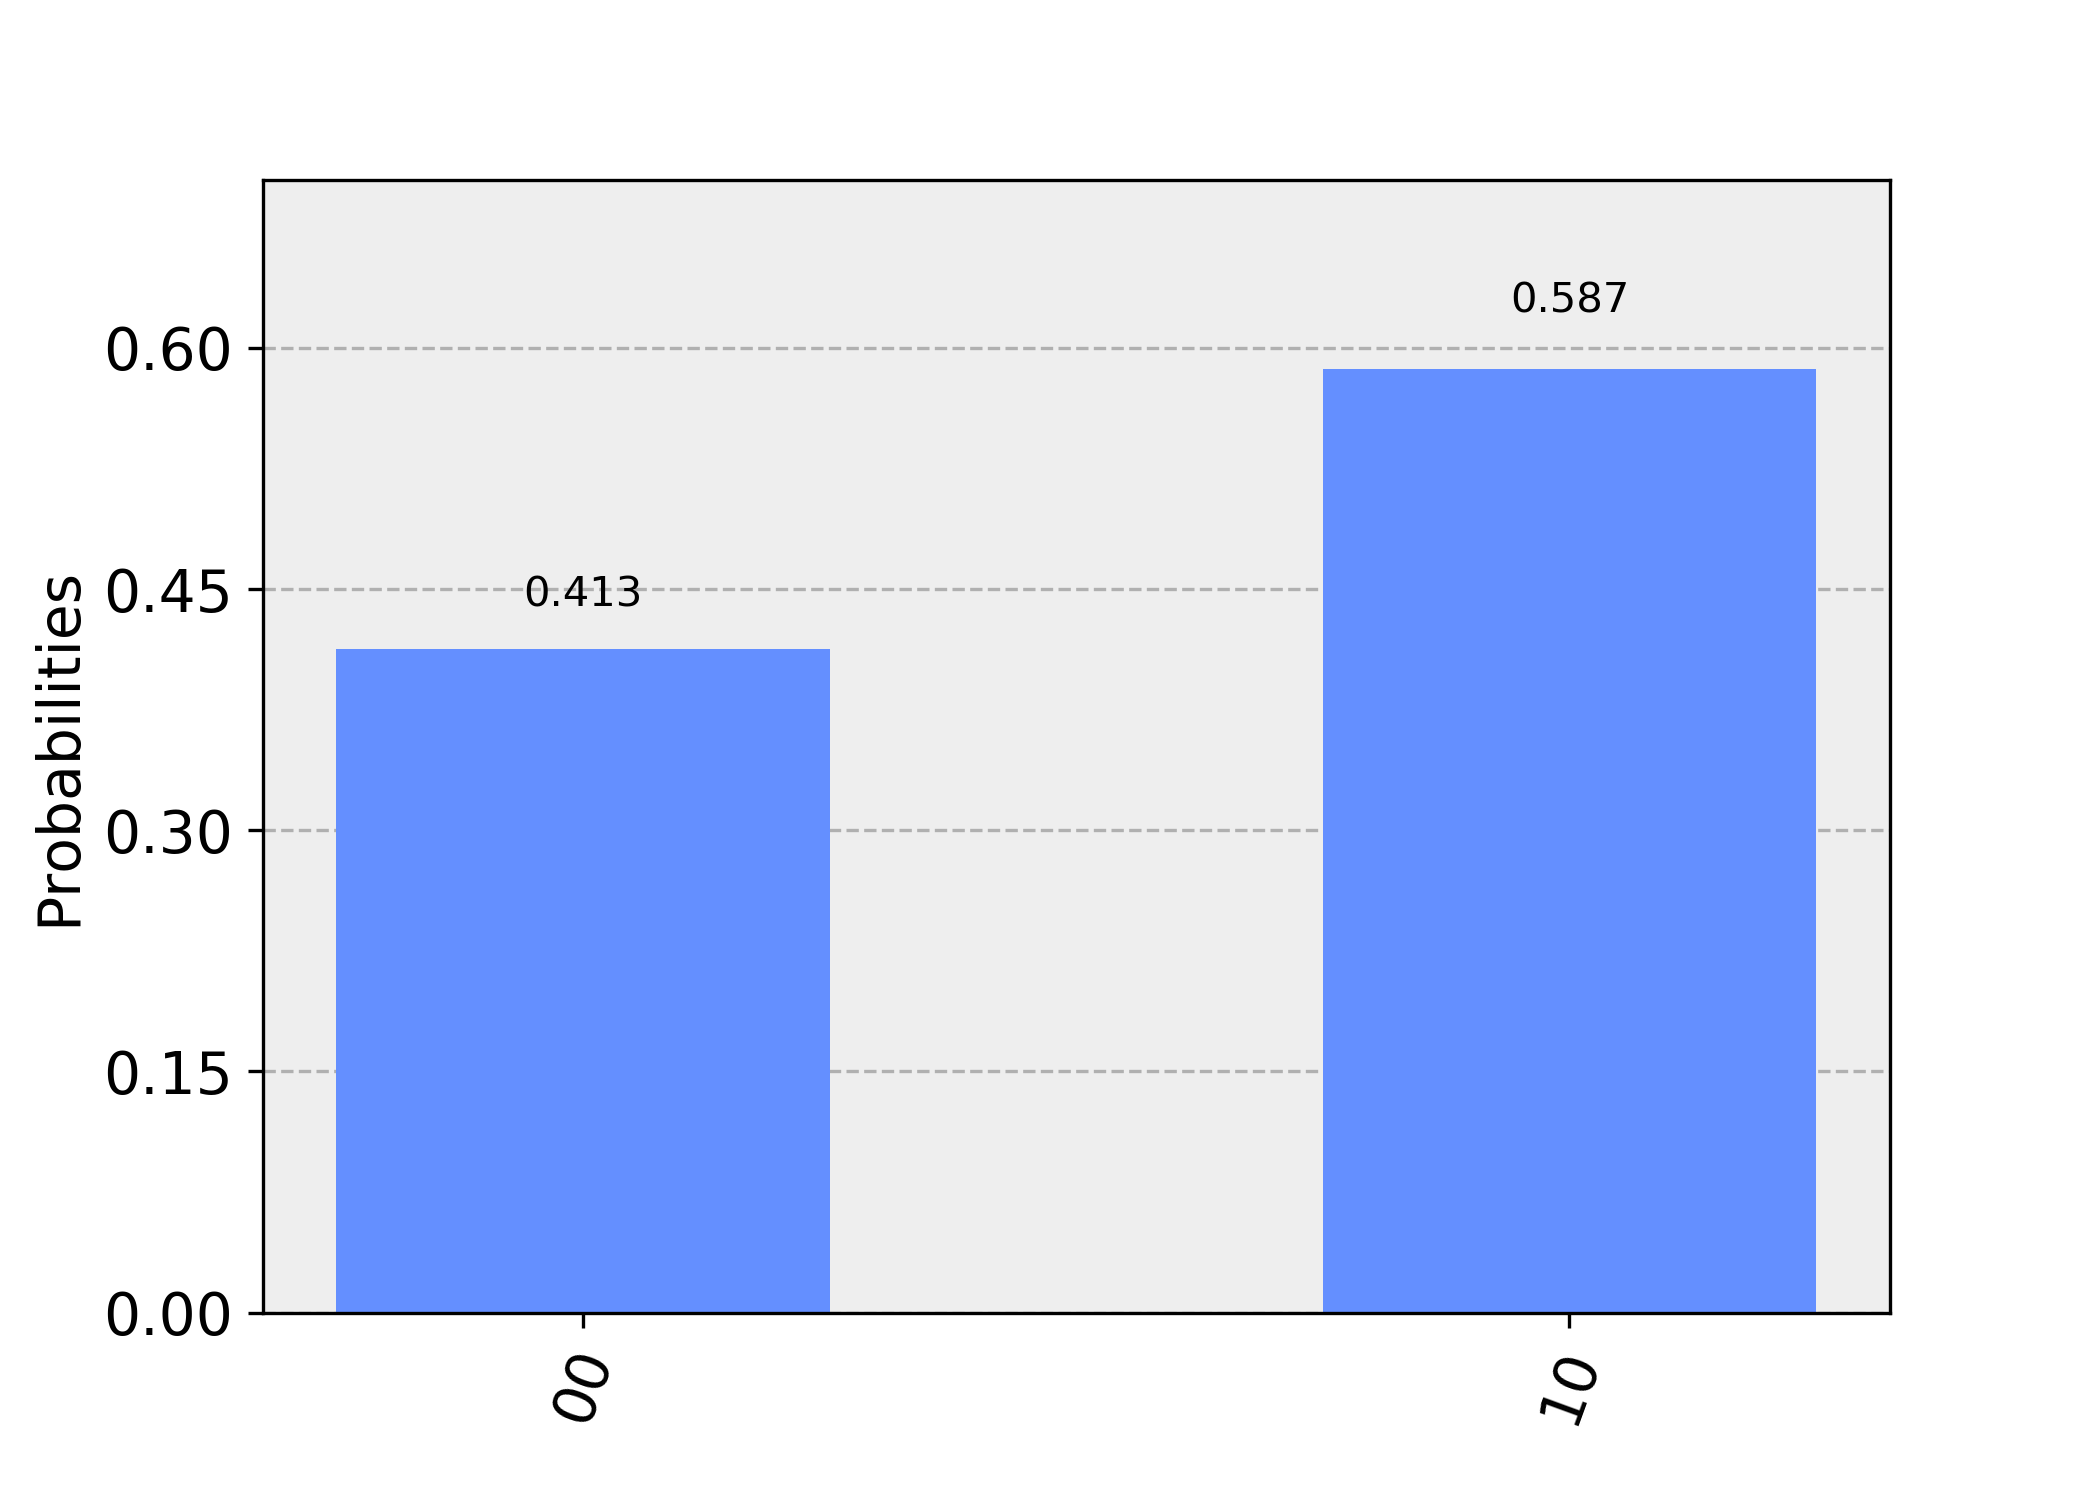
\includegraphics[width=\linewidth]{gfx/misura_versicolor_filtrata}
    }
    \caption{Simulazione del circuito, risultati filtrati}
    \label{fig:simulazione_filtrati}
\end{figure}

Il passo successivo è eseguire questi stessi circuiti quantistici su un vero computer quantistico. 
È stata scelta la macchina a 16 qubit ibmq\_16\_melbourne per ottenere le misure per il 
vettore d'input setosa illustrate in figura \ref{fig:sperimentale_setosa}. 
Gli inevitabili fenomeni di rumore rendono i risultati meno piccati ma comunque 
distinguibili. 

\begin{figure}[h!]
    \centering
    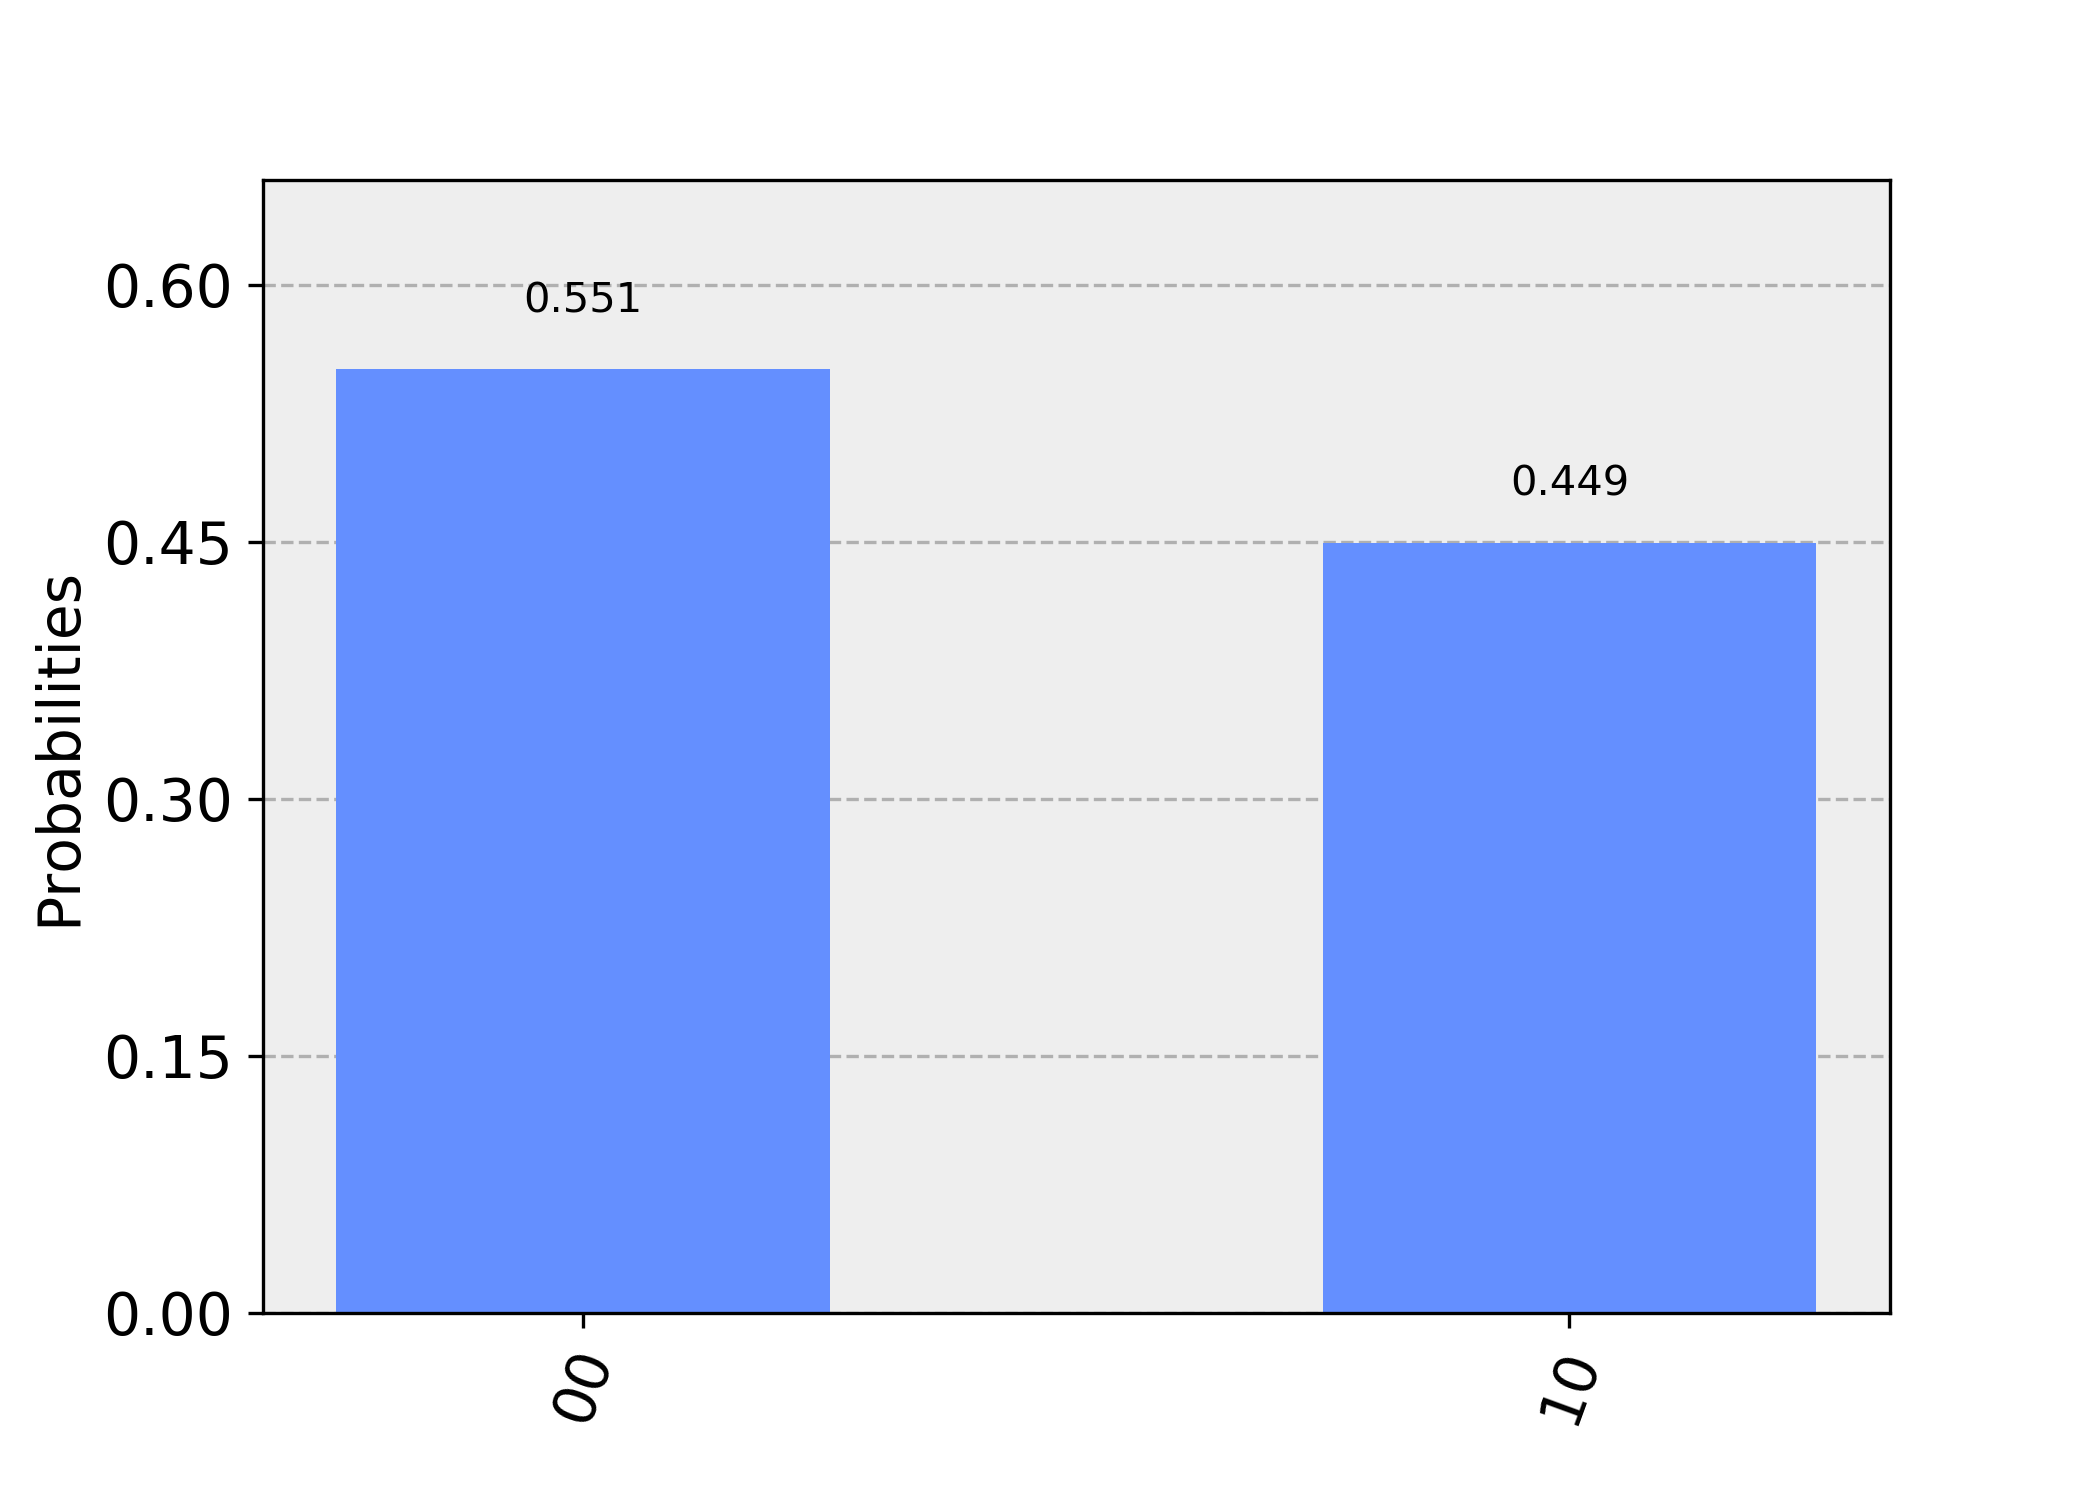
\includegraphics[width=\linewidth]{gfx/misura_setosa_sperimentale}
    \caption{Esecuzione su hardware reale (setosa)}
    \label{fig:sperimentale_setosa}
\end{figure}

Il discorso è diverso per il confronto tra le classi versicolor e 
virginica: visto che gli elementi di queste due classi non sono linearmente 
separabili, algoritmi come il \ac{KNN} non sono efficaci nella loro distinzione. 
Infatti le misure effettuate danno risultati erronei o 
ambigui nella maggioranza dei casi (probabilità del 50\% per entrambi i risultati). 
Uno dei metodi per aggirare questo problema è l'uso di feature map 
\cite{schuld} nel processo di ottimizzazione. 

% Ad ogni modo, si procederà nel realizzare i punti definiti all'inizio di 
% questo capitolo. Condizione necessaria per distinguere le tre classi con un 
% solo esperimento è che si possano memorizzare almeno tre vettori di training, 
% uno per ciascuna classe. 

\section{Limiti di esecuzione}

Nell'esecuzione dell'algoritmo su hardware quantistico si è dovuto tenere 
conto dei limiti in termini di numero di qubit. Il computer quantistico 
disponibile tramite IBM Q Experience permette di usare al massimo 
14 qubit superconduttivi. Considerando che, per ogni qubit di controllo aggiuntivo, 
la porta $C^n R_y (\theta)$ richiede un ulteriore qubit ancilla, la spesa 
in termini di risorse è di due qubit per ogni incremento tra numero di vettori 
di training, di classi o di caratteristiche. Alcune configurazioni ottimali 
per l'esecuzione con 14 qubit sono descritte in tabella \ref{table:conf.ottimali}. 
Si ricorda che dato un registro di $n$ qubit, questo può conservare $N=2^n$ 
valori nelle sue ampiezze di probabilità. 

\begin{table}[h!]
    \centering
    \begin{tabular}{c c c}
        i & m & c \\ 
        \hline
        2 & 2 & 2 \\ 
        3 & 2 & 1 \\ 
        2 & 3 & 1 \\ 
        1 & 3 & 2
    \end{tabular}
    \caption{Alcune configurazioni per i qubit}
    \label{table:conf.ottimali}
\end{table}

Un'esecuzione che sfrutti due qubit classe, tre qubit indice e un qubit caratteristica 
necessita di 5 qubit ancilla ed un qubit registro per la costruzione della \ac{QRAM}, 
un qubit ancilla per il \ac{QKNN}, per un totale di 13 qubit. Una classificazione di 
questo tipo è stata eseguita sul processore quantistico ibm\_16\_melbourne: si sono 
confrontati vettori d'input casuali presi dalle tre classi con insiemi di apprendimento 
allo stesso modo costruiti casualmente, avendo cura di inserire in maniera uniforme 
elementi delle diverse classi. Con 3 qubit $\ket{m}$ abbiamo a disposizione 8 vettori di 
apprendimento; l'insieme di training possiede 2 vettori dalla classe setosa, 3 da versicolor 
e 3 da virginica. Si riportano in figura \ref{fig:classificazione.reale} i 
risultati (filtrati, come fatto precedentemente) di classificazione di un elemento 
della classe setosa; il circuito è stato eseguito 8192 volte e l'istogramma riporta 
la probabilità che il vettore d'input appartenga ad una determinata classe, 
come evidenziato nell'eq. \ref{eq:prob.classe}. L'esito di classificazione è rappresentato 
dai due bit a sinistra, mentre i due bit a destra assicurano l'esecuzione delle misure 
condizionali $\ket{a} = \ket{0}$ e $\ket{j}_R = \ket{1}_R$. 
La classe setosa è legata al risultato di 
misura $\ket{c} = \ket{00}$, versicolor a $\ket{c} = \ket{01}$ e virginica a $\ket{c} = \ket{10}$; 
lo stato $\ket{c} = \ket{11}$ resta inutilizzato. 

% ************************************************
% Inserire risultati di esecuzione su hardware reale
% ************************************************

\begin{figure}[h!]
    \centering
    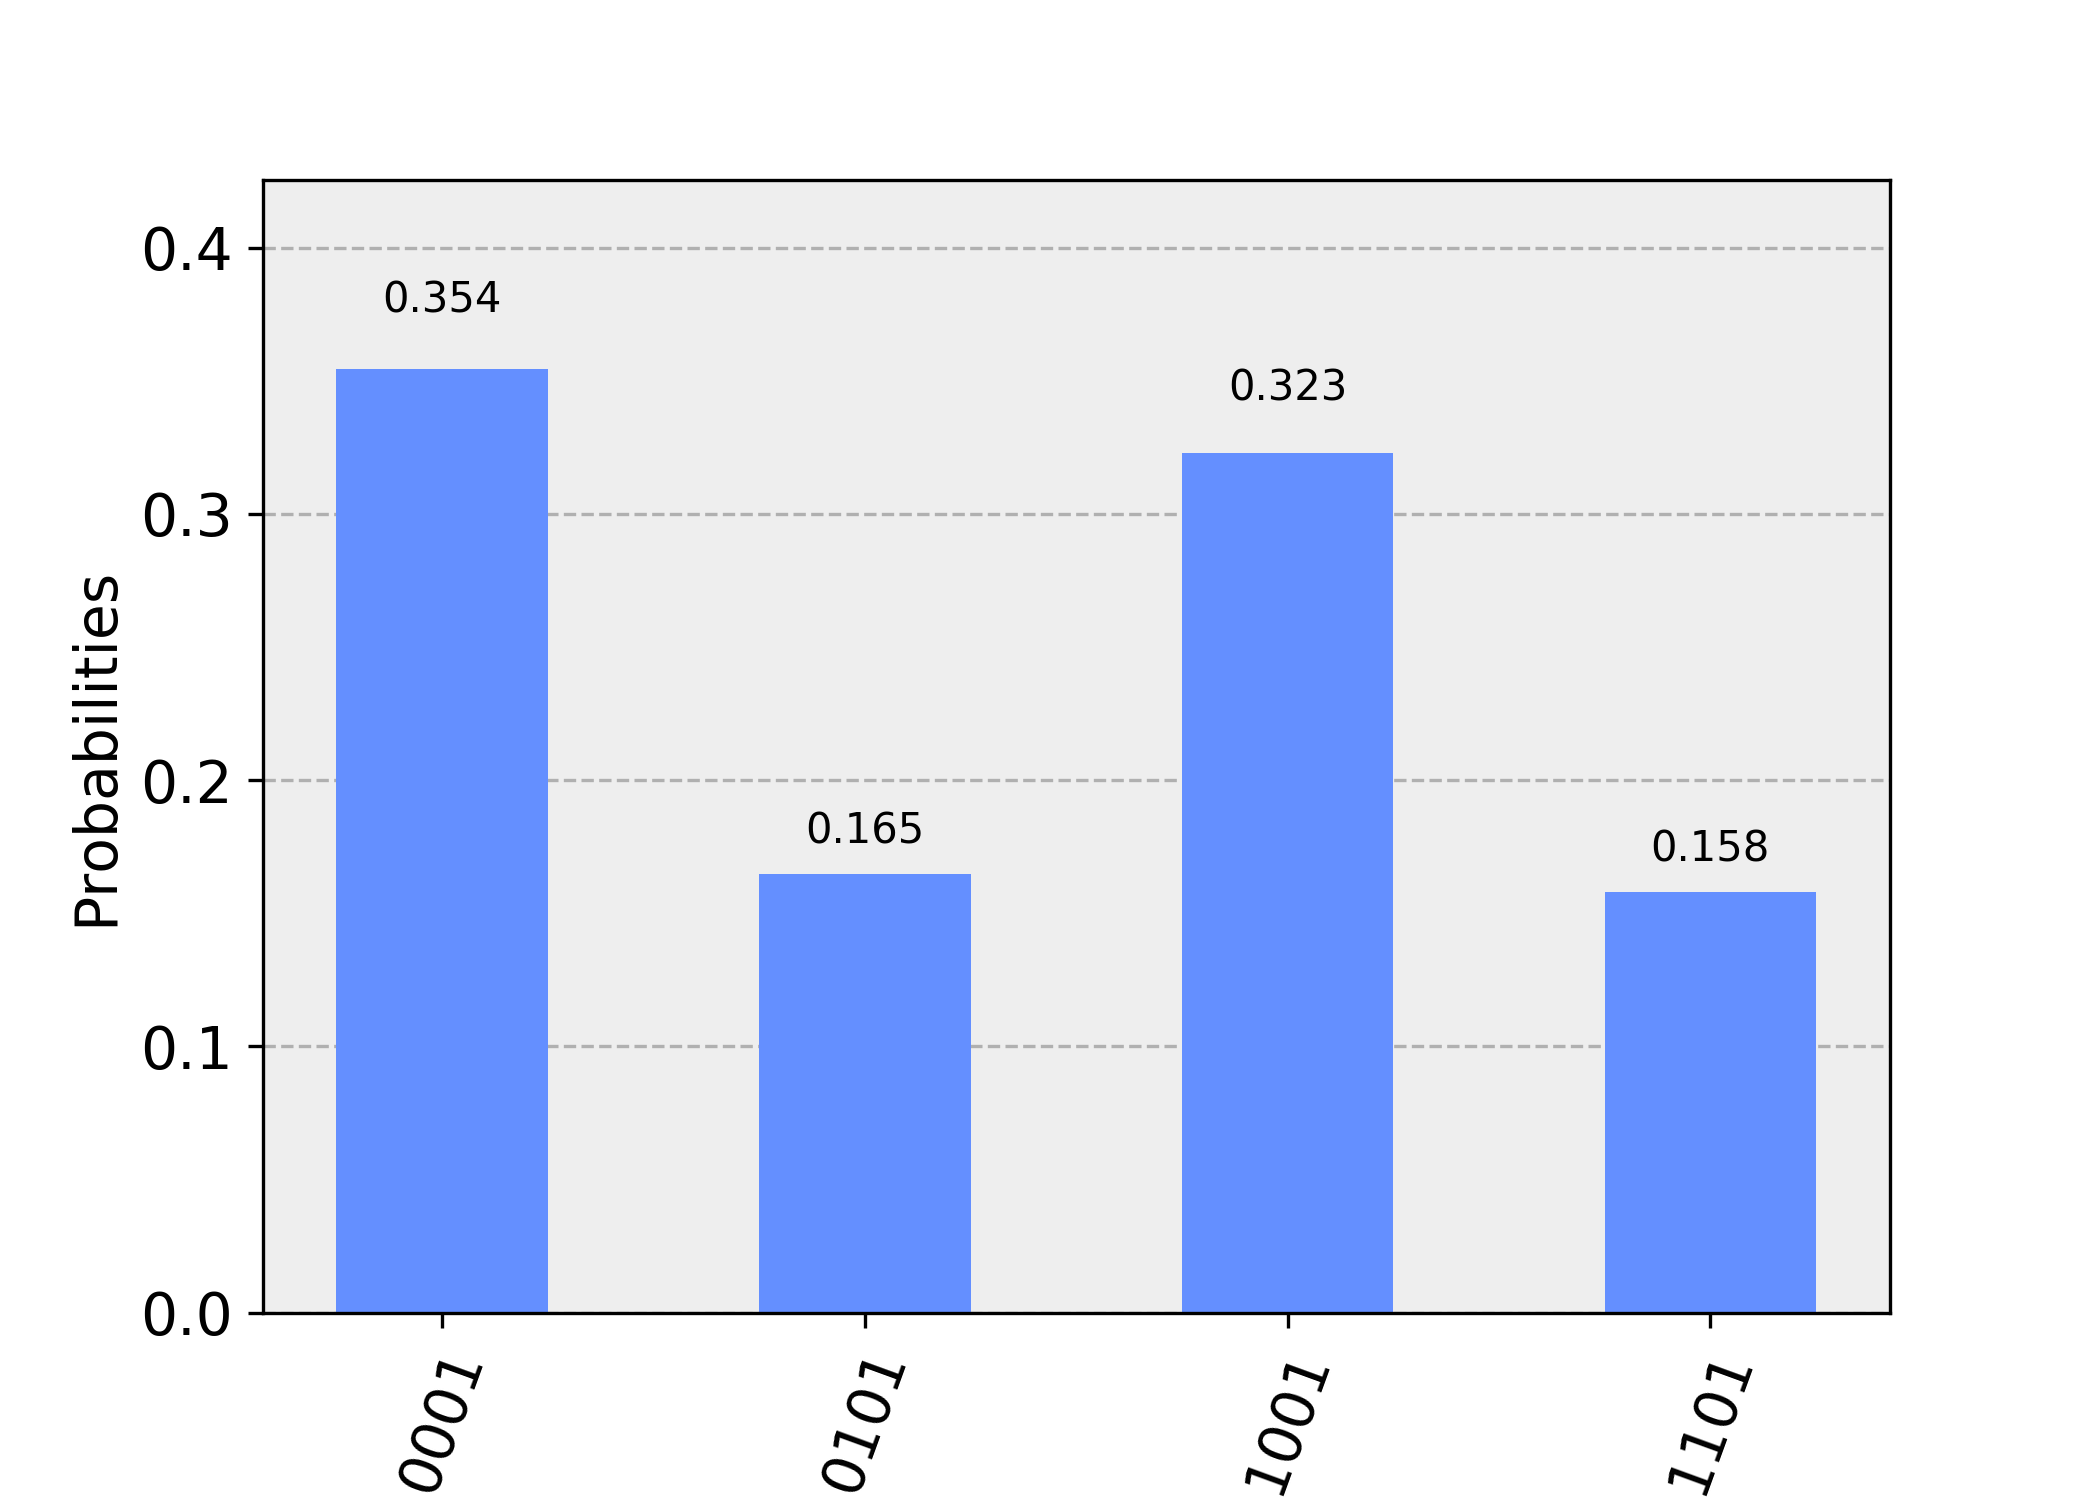
\includegraphics[width=\linewidth]{gfx/setosa_reale_20190913:1716}
    \caption{Risultati sperimentali multiclasse (setosa)}
    \label{fig:classificazione.reale}
\end{figure}

Si può notare come nell'esecuzione su hardware reale si presentino disturbi legati 
agli inevitabili fenomeni di decoerenza, dati dal grande numero di porte usate; 
tra i risultati di esecuzione sperimentale è capitato infatti che i vettori setosa 
fossero erroneamente classificati come virginica, in un numero piccolo ma non 
insignificante di volte. 
Basti confrontare i risultati sperimentali con quelli di esecuzione simulata usando gli 
stessi vettori d'input e di training in figura \ref{fig:classificazione.multiclasse.simulata} per rendersi 
conto dell'effetto non trascurabile delle interazioni ambientali sui qubit.
Non sono disponibili dati in merito al tempo di esecuzione effettivo sul processore, 
in quanto l'informazione non viene più fornita nella versione del software in uso 
mentre si scrive questa tesi. Tenendo conto del tempo di attesa in coda, il tempo totale 
può andare da mezz'ora alle due ore in media. 

\begin{figure}[h]
    \centering
    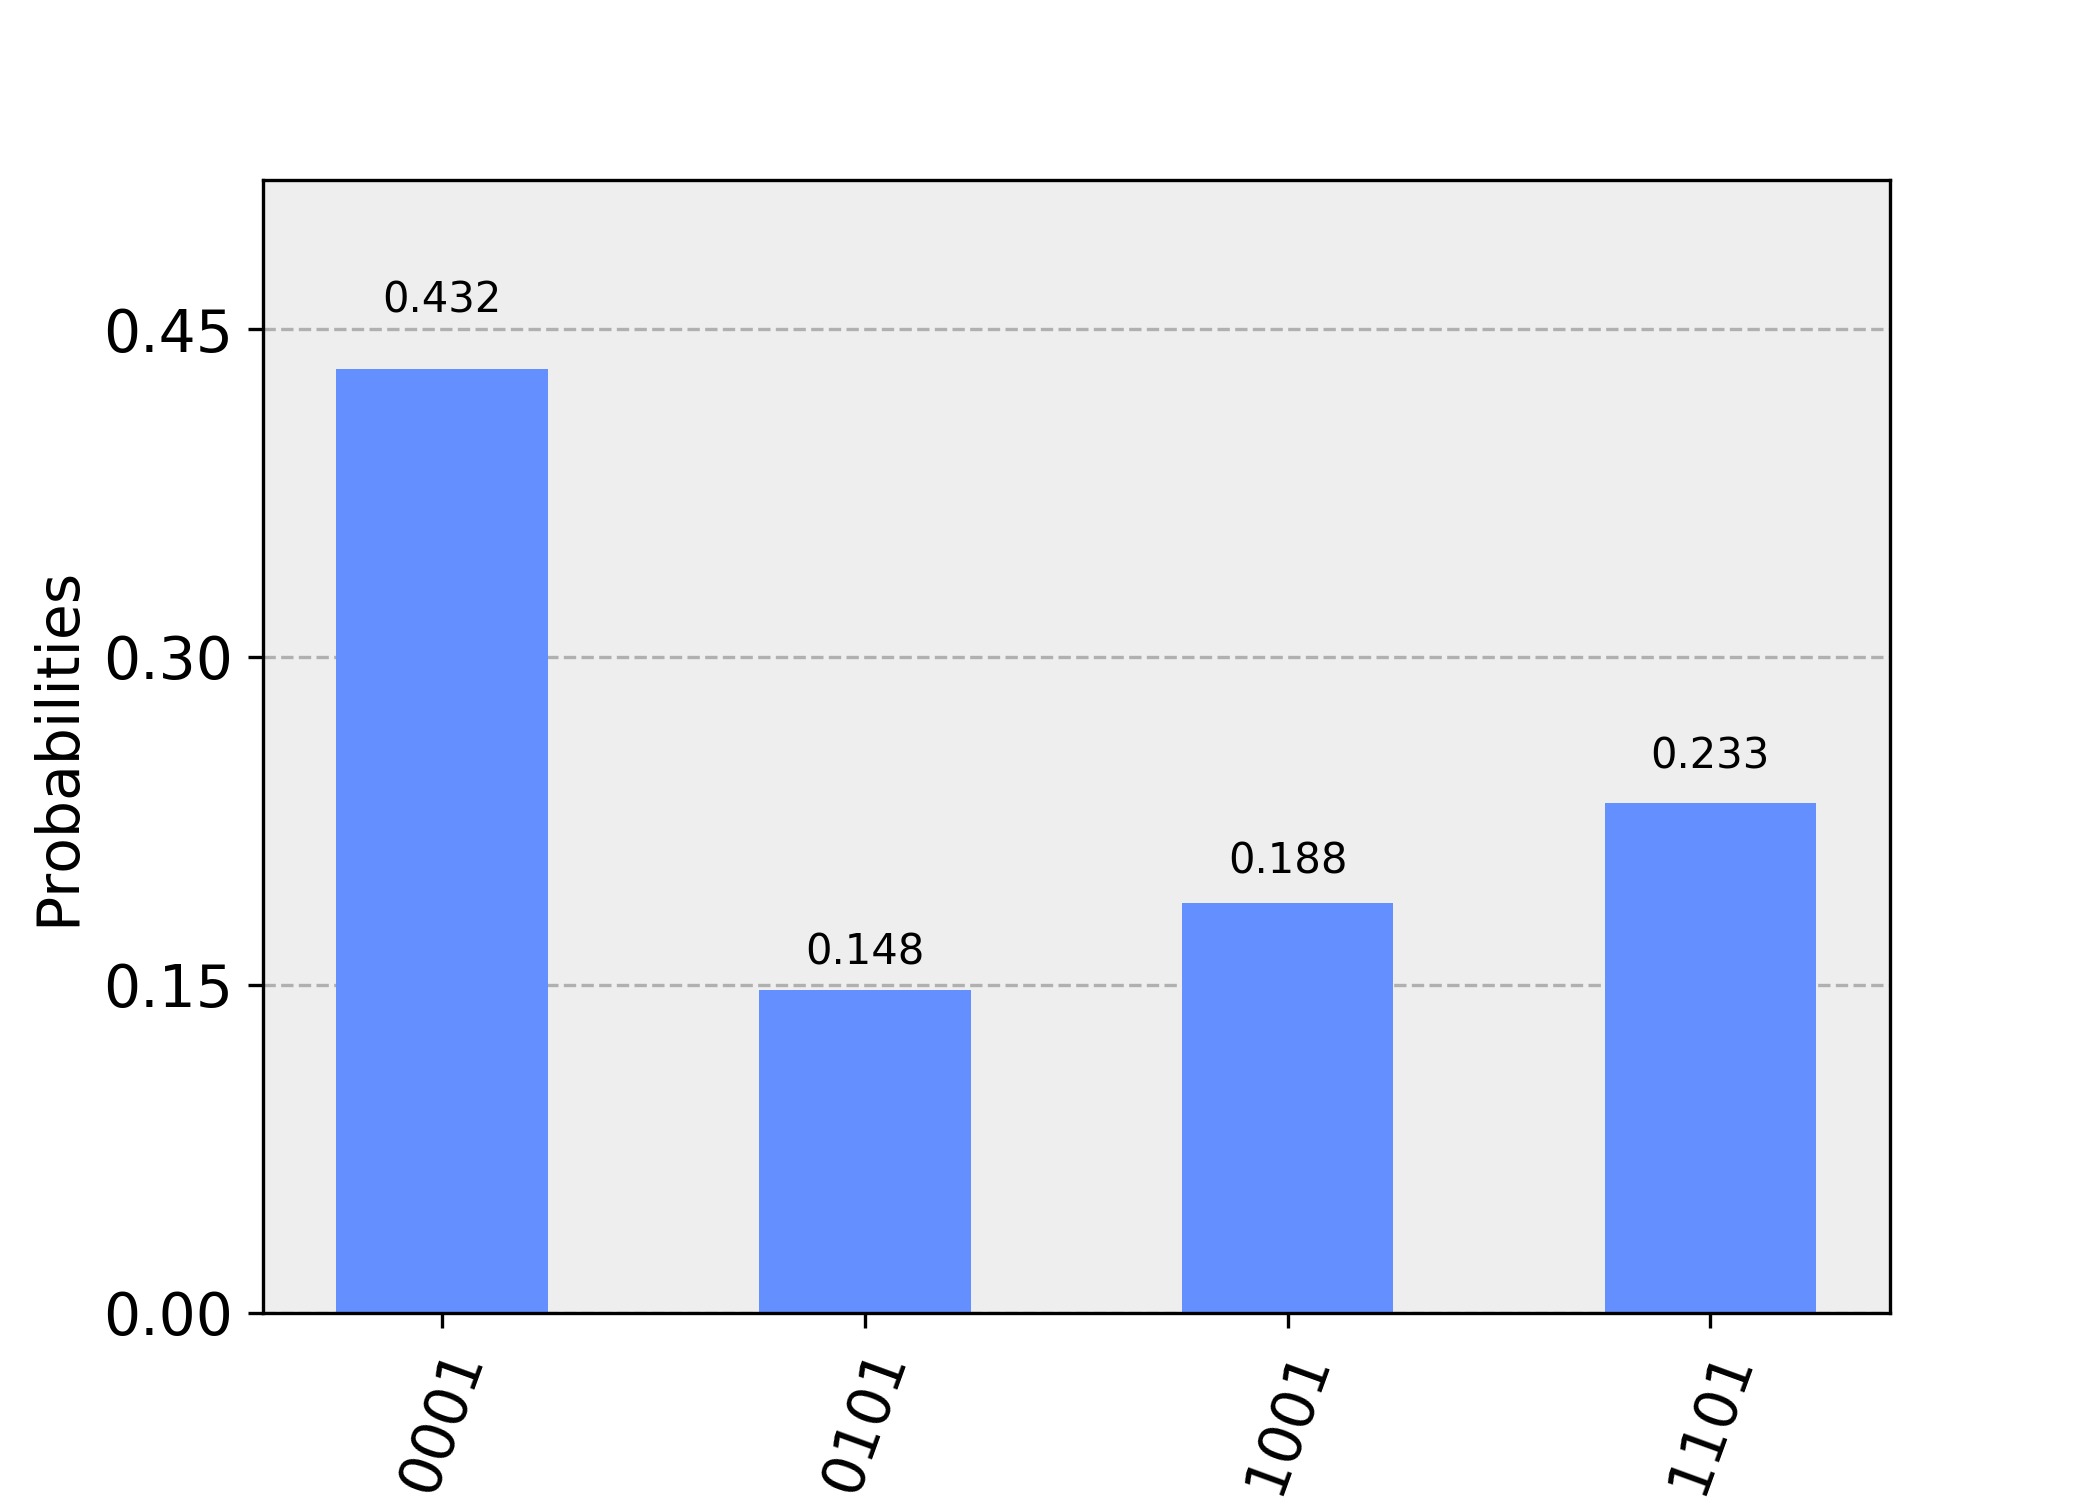
\includegraphics[width=\linewidth]{gfx/setosa_simulato_multiclasse.png}
    \caption{Risultati simulati multiclasse (setosa)}
    \label{fig:classificazione.multiclasse.simulata}
\end{figure}

% *********************************************
% Questa parte va aggiustata
% *********************************************

% Per verificare il miglioramento apportato da un aumento del numero di caratteristiche, 
% si prende in esame la classificazione del vettore d'input 54 (versicolor), 
% con i vettori di training numero 51 (versicolor) e 146 (virginica) del data set. 
% Il vettore d'input viene classificato correttamente durante la simulazione con due caratteristiche, 
% con probabilità vicina al 51.4\%. 
% Effettuando la stessa misura, ma tenendo conto di tutte le quattro feature, arriviamo ad 
% una probabilità di classificazione corretta del 58.3\% nel migliore dei casi. 
% Sembra esserci un margine di miglioramento in determinati casi, 
% ma non può essere garantito in maniera generale. 

% Per studiare l'efficienza dell'algoritmo a diversi stadi di miglioramento, 
% si divide il data set in un insieme dedicato all'addestramento ed un insieme 
% di vettori da classificare. Al fine di avere risultati imparziali, 
% per ogni esecuzione i vettori di training ed il vettore d'input 
% sono scelti casualmente a partire dal data set completo. 
% Si contano le classificazioni di successo 
% rispetto al totale dei tentativi, al variare dei parametri come il numero 
% di features o il numero di vettori di training usati. 

Per verificare l'efficienza dell'algoritmo con maggiori risorse, si sono eseguiti 
vari tentativi di classificazione con circuiti simulati, al variare del numero di 
vettori di training. In tabella \ref{table:misure} si possono trovare i relativi 
risultati, dove si intende che per ogni esperimento si è costruito un circuito 
che accettasse insiemi casuali di vettori dal data set ed è stato eseguito 8192 
volte, dopo di che si sono rimescolati gli insiemi di training e si è rieseguito 
l'esperimento per 10 volte in totale. 

\begin{table}[h!]
    \centering
    \begin{tabular}{c c c}
        classe & $m=5$ & $m=7$ \\ 
        \hline
        setosa & 100\% & 100\%\\ 
        versicolor & 50\% & 80\%\\ 
        virginica & 90\% & 90\%
    \end{tabular}
    \caption{Risultati positivi di classificazione con $2^m$ vettori di training}
    \label{table:misure}
\end{table}

I risultati vengono necessariamente da simulazioni, in quanto sono necessari 
23 qubit per il caso con $m=7$ qubit. Un esempio di simulazione di classificazione 
positivo, in quanto con $2^7=128$ vettori di training è usato quasi tutto il data set, 
per la classe virginica è visibile in figura \ref{fig:multiclasse}. 

\begin{figure}[h!]
    \centering
    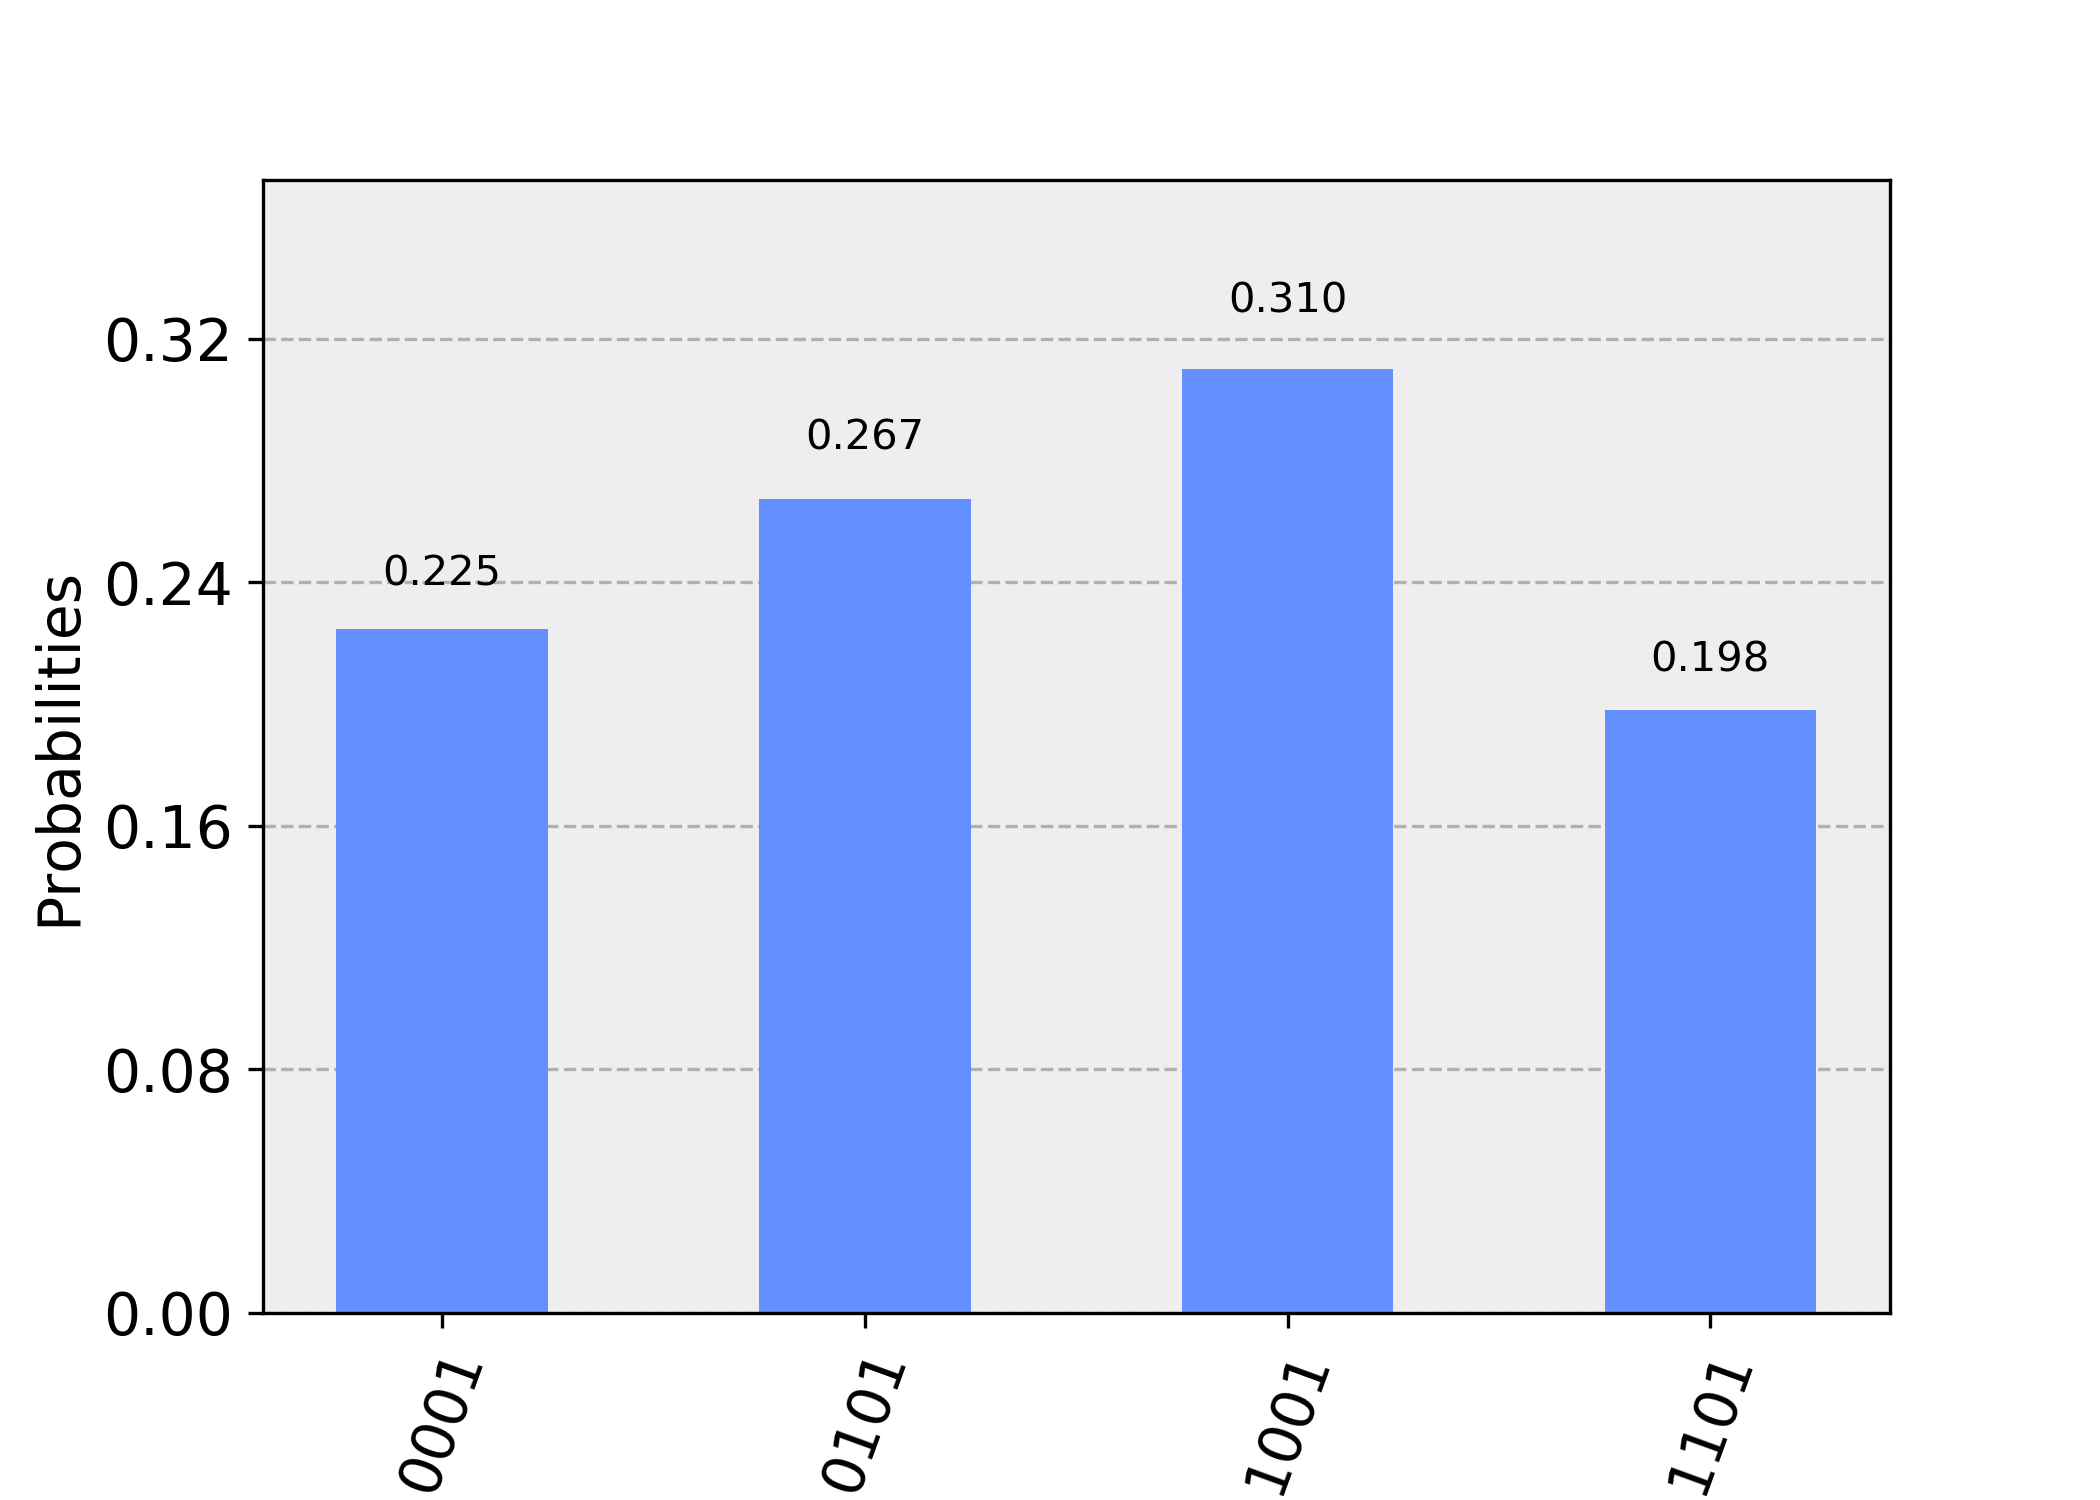
\includegraphics[width=\linewidth]{gfx/multiclass_virginica}
    \caption{Classificazione di virginica multiclasse}
    \label{fig:multiclasse}
\end{figure}

Si fa presente che l'uso di tecniche di preprocessing avrebbero permesso di 
distinguere le classi versicolor e virginica con ben meno vettori di training, 
tuttavia uno tra gli scopi di questa tesi era verificare fino a che punto si possono 
immagazzinare vettori in quantità sempre maggiori ai fini della classificazione 
ed ottenere i risultati aspettati. 

\section{Un esempio più semplice}

Per ottenere dei risultati più chiari, si è effettuata la classificazione 
anche su un data set semplificato, formato da vettori bidimensionali 
appartenenti a quattro classi, disposti in cluster ben separati tra loro. 

\begin{figure}[h!]
    \centering
    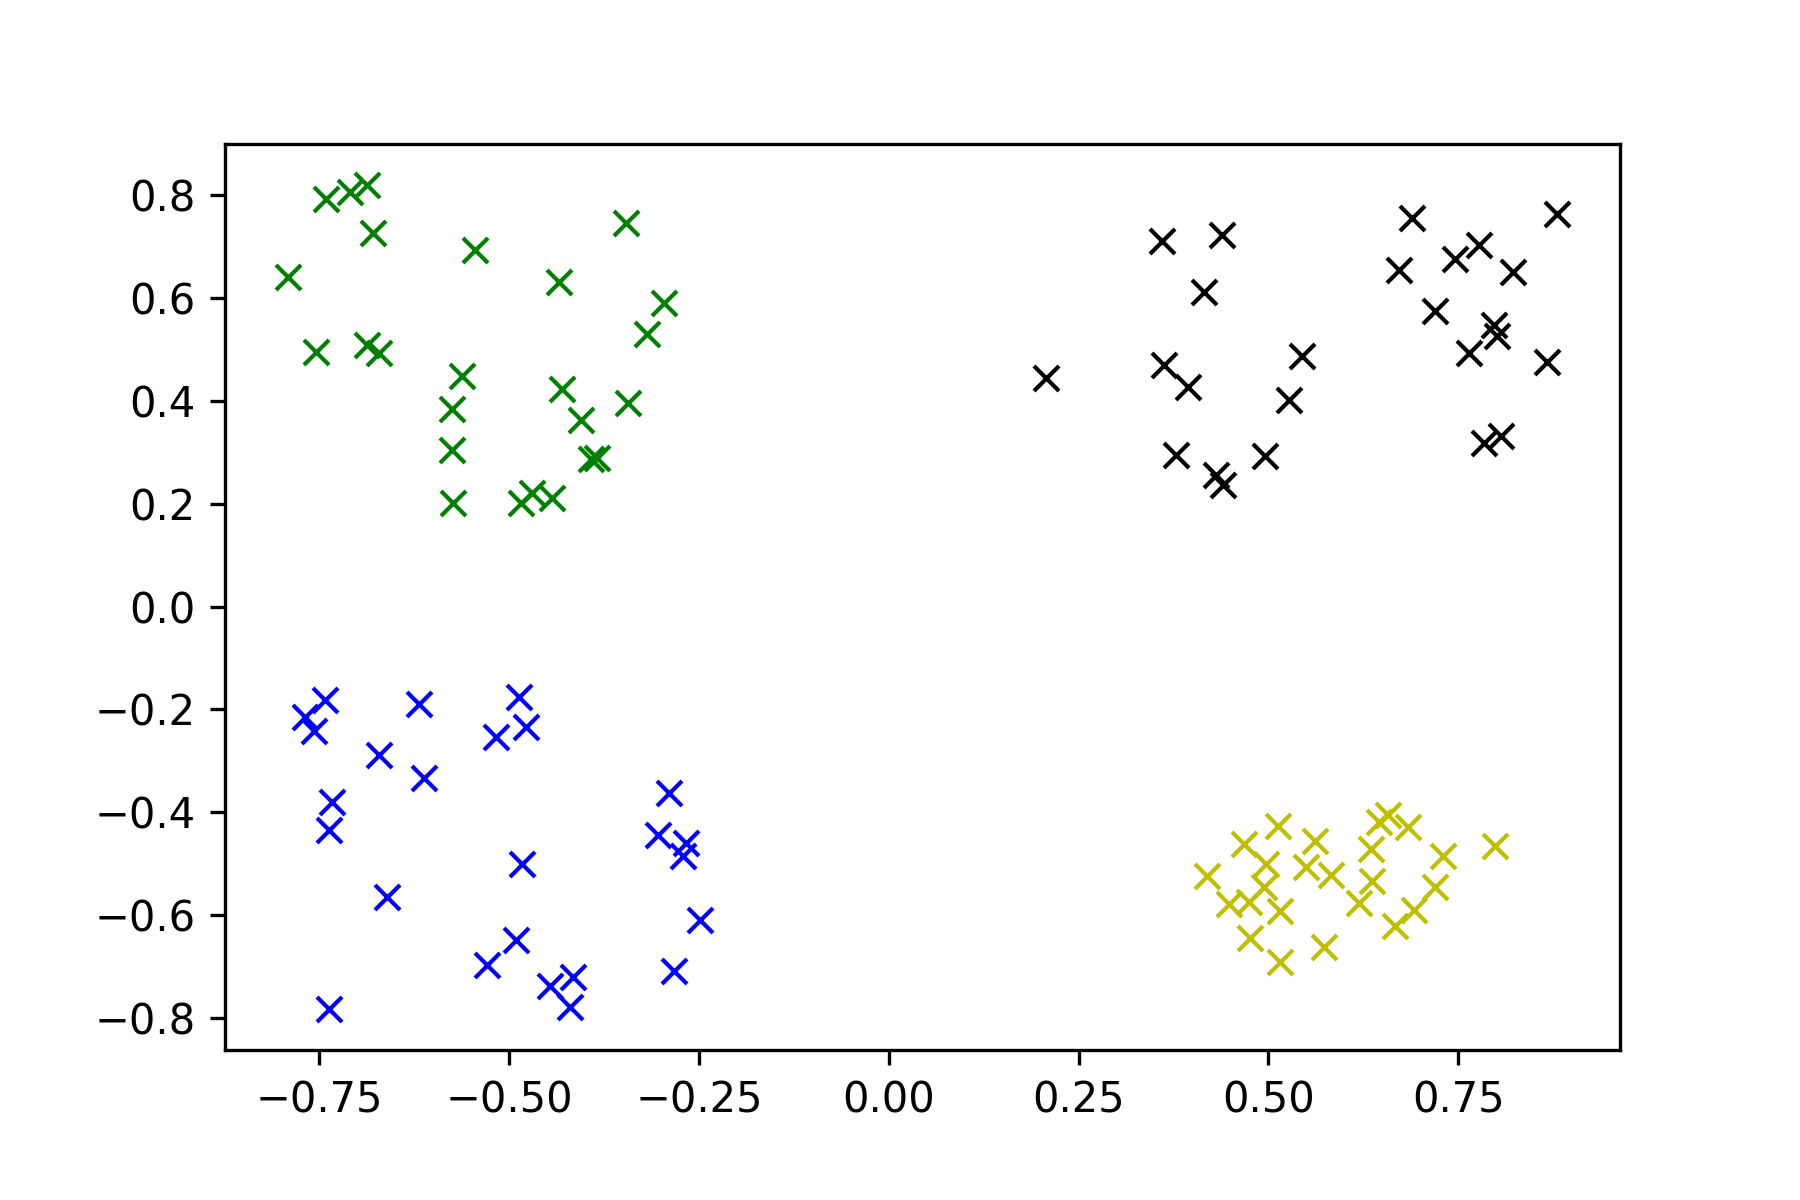
\includegraphics[width=\textwidth]{gfx/cluster/cluster}
    \caption{Data set a cluster}
    \label{fig:cluster}
\end{figure}

Usando lo stesso procedimento visto nella sezione precedente, si sono 
selezionati due elementi da ciascun cluster ed li si è etichettati con un colore; 
si è poi confrontato in quattro esecuzioni separate un terzo vettore 
casuale da ciascun gruppo.\footnote{Si veda \cite{anagolum} per una versione 
one vs. all in cui vengono implementati $n$ classificatori quantistici binari di questo tipo, 
dove $n$ è il numero di classi.}

\begin{figure}[h!]
    \centering
    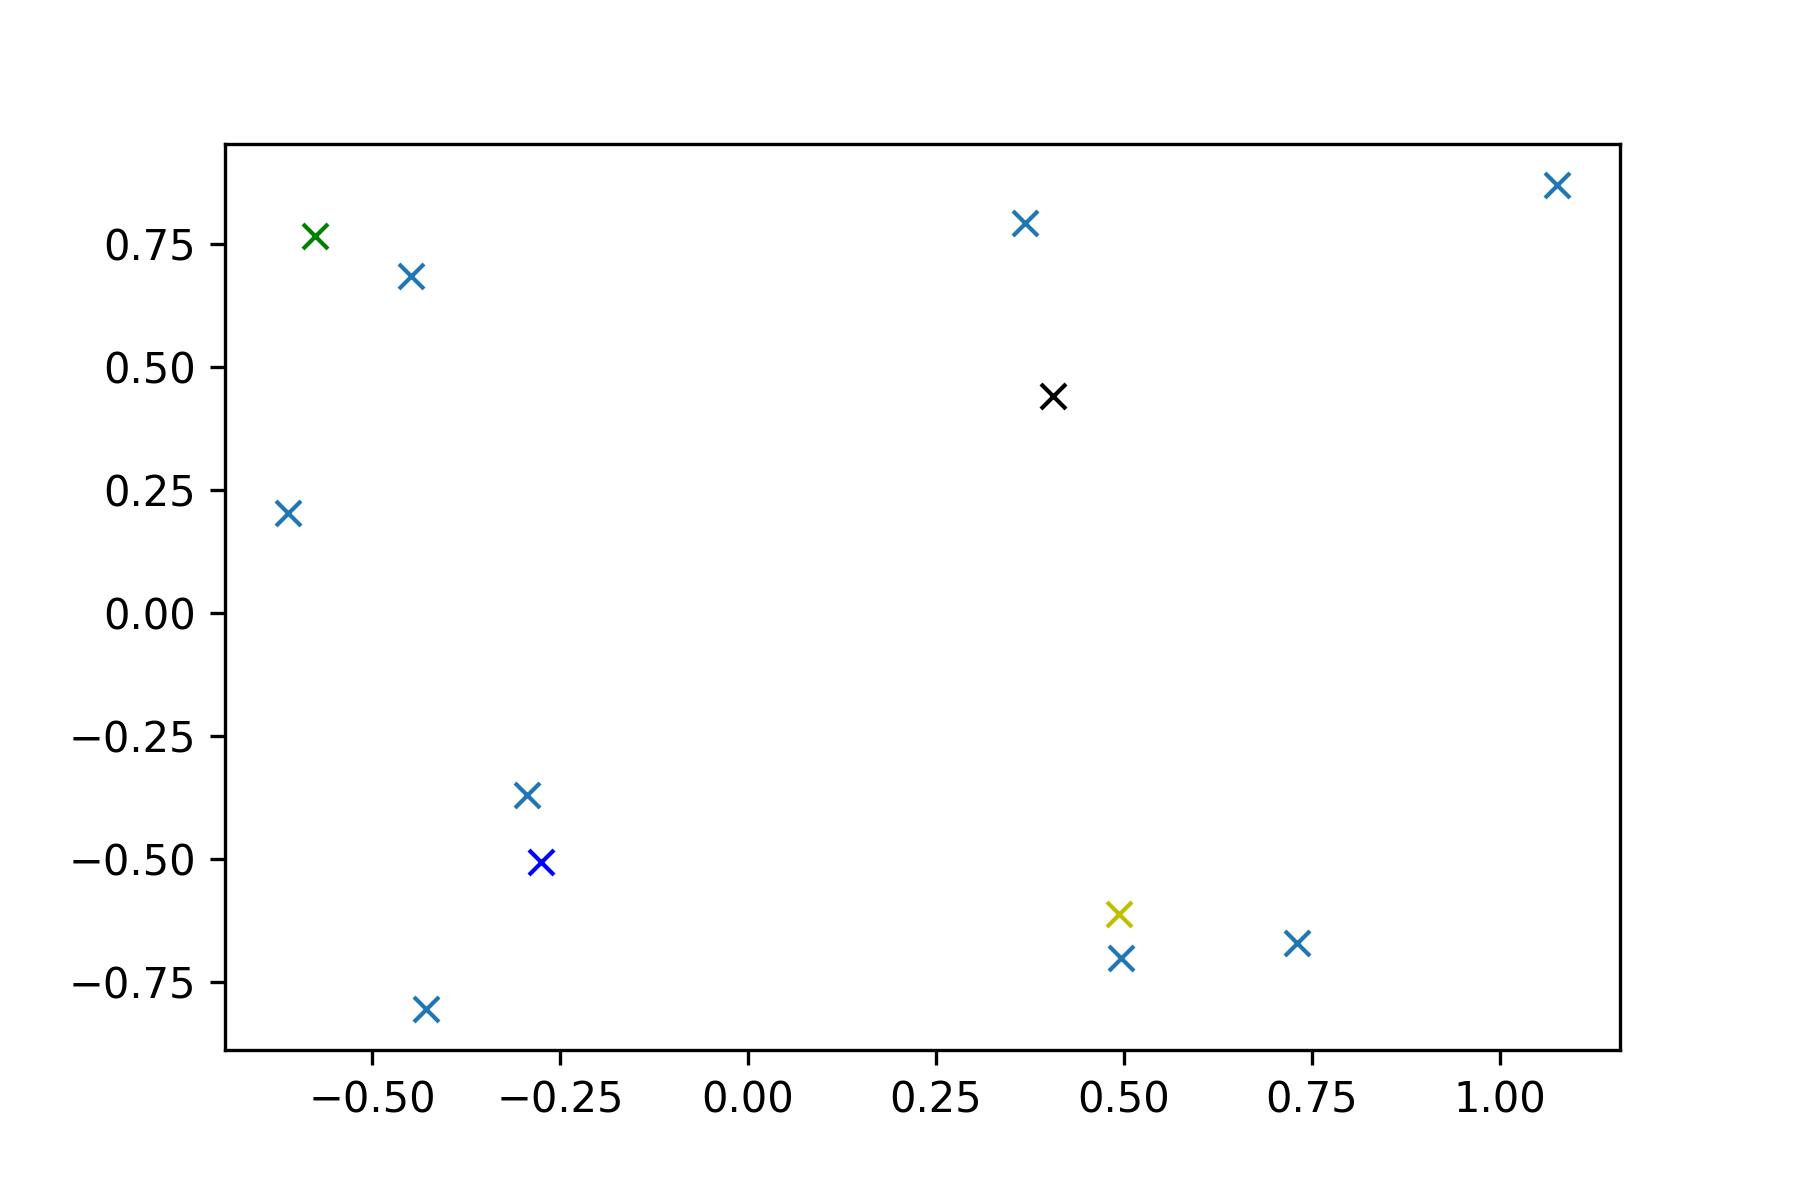
\includegraphics[width=\textwidth]{gfx/cluster/random}
    \caption{Vettori casuali dopo l'applicazione di arcoseno}
    \label{fig:random}
\end{figure}

I risultati di simulazione vengono presentati nel riquadro \ref{fig:cluster.simulazione}, 
quelli di esecuzione su hardware reale non sono disponibili per mancanza di tempo 
dovuta alle scadenze di consegna della tesi. 

\begin{figure}[h!]
    \myfloatalign
    \hspace{-0.30\linewidth}
    \subfloat[Classe verde]
    {\includegraphics[width=.60\linewidth]{gfx/cluster/Simulated/green}} \quad
    \subfloat[Classe blu]
    {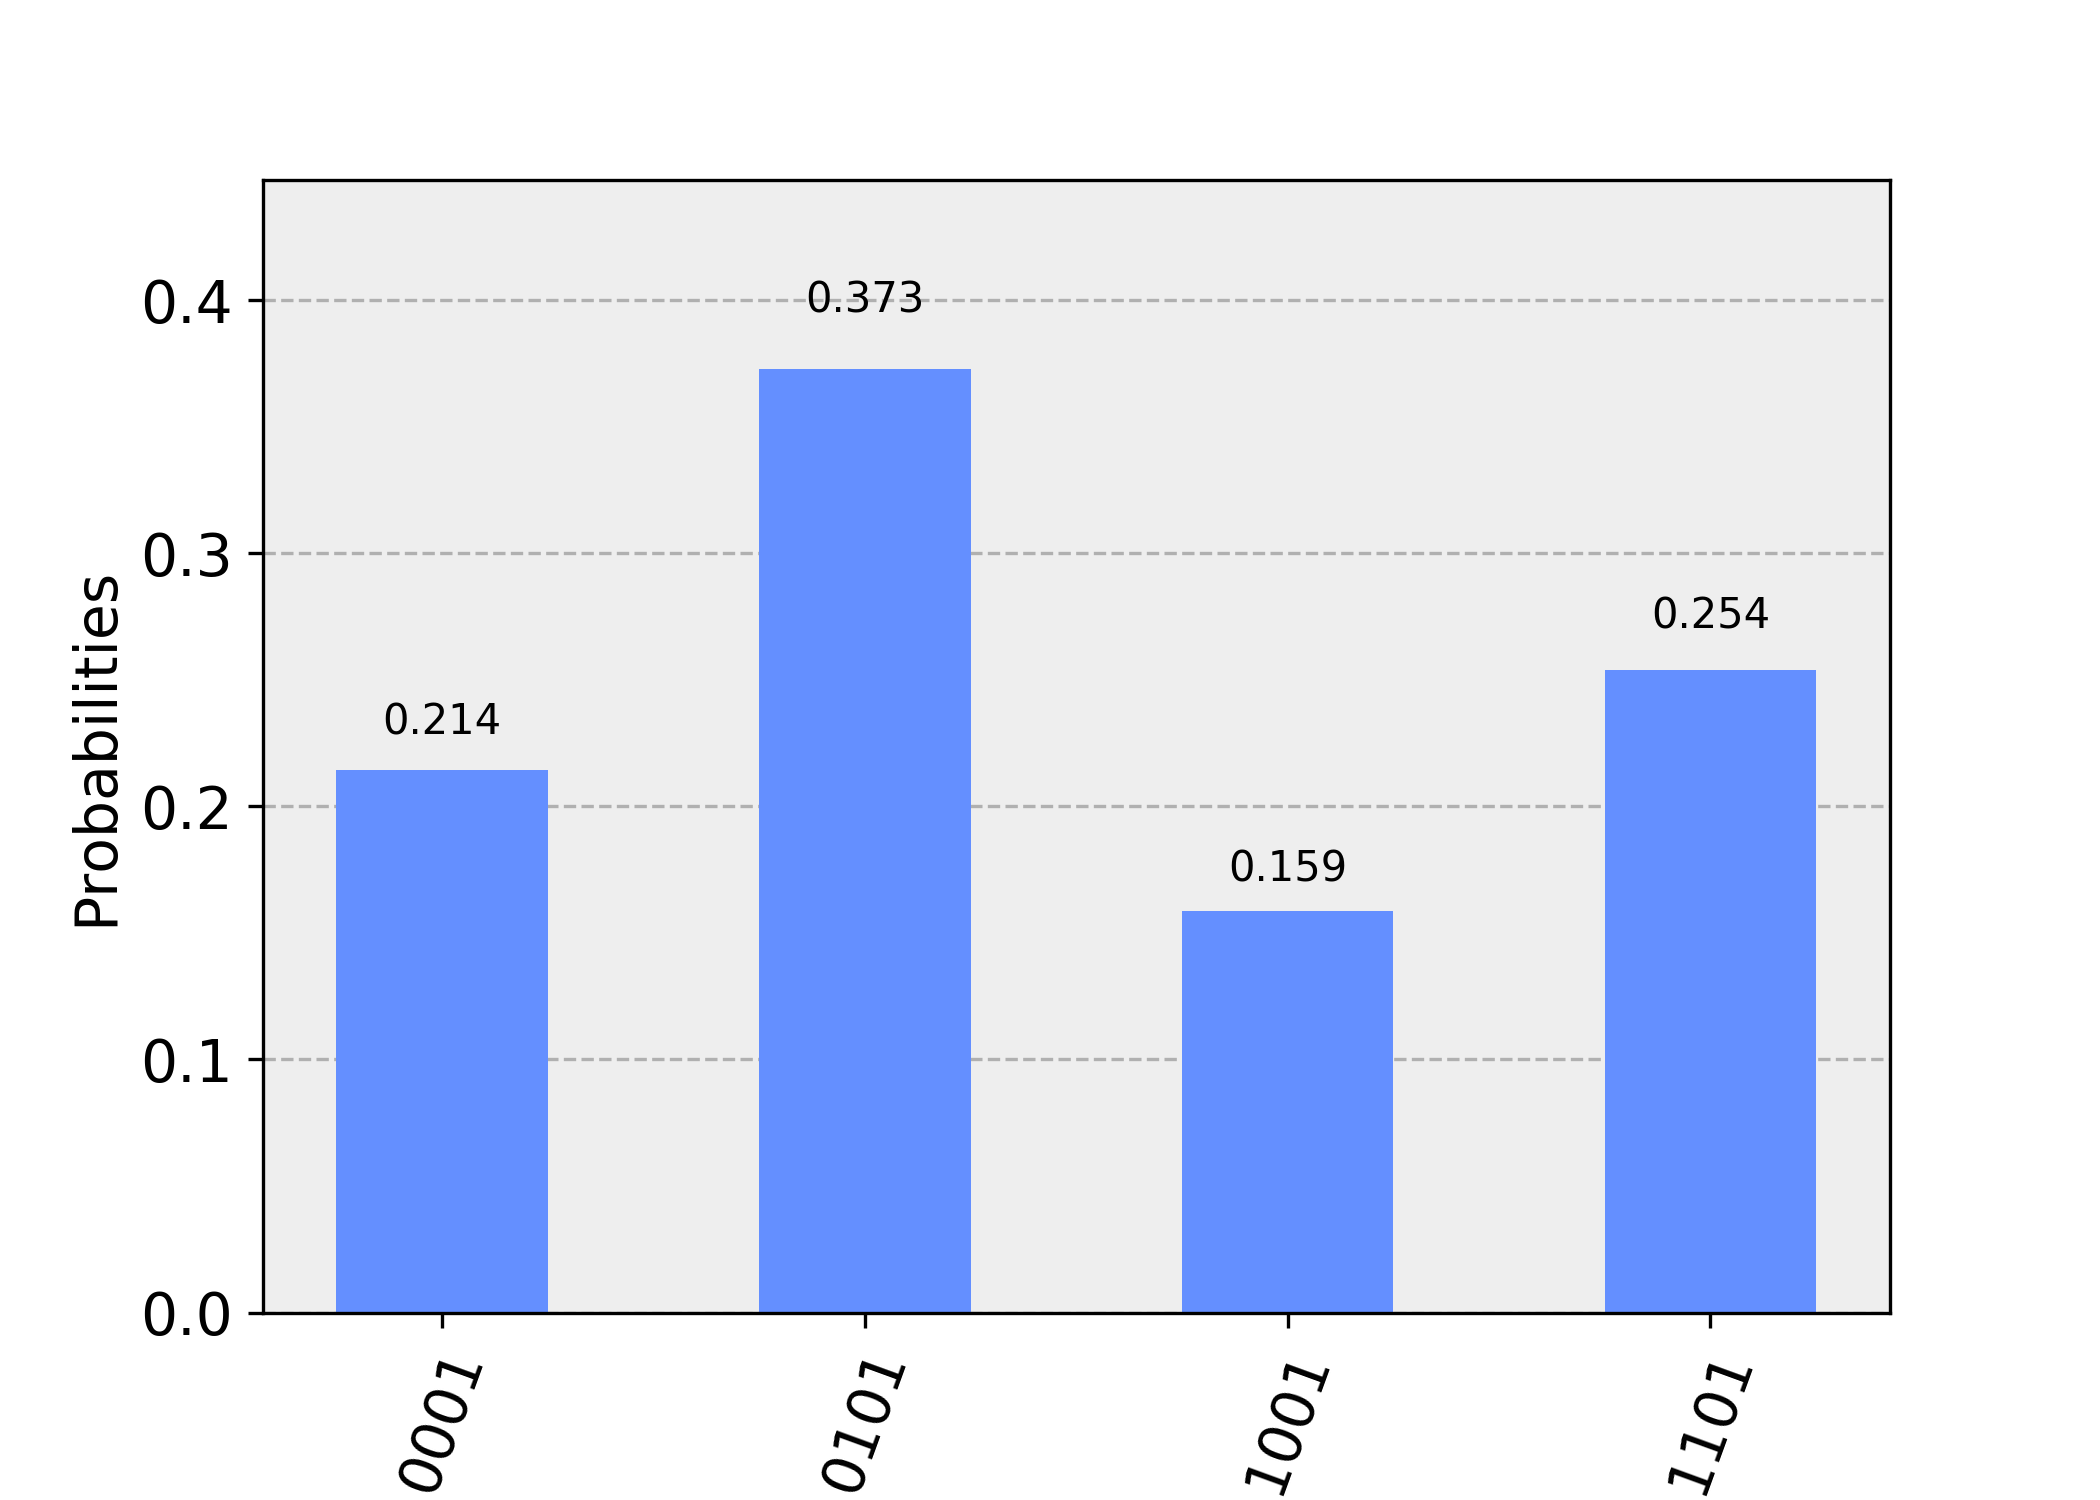
\includegraphics[width=.60\linewidth]{gfx/cluster/Simulated/blue}} \\
    \hspace{-0.30\linewidth}
    \subfloat[Classe nera]
    {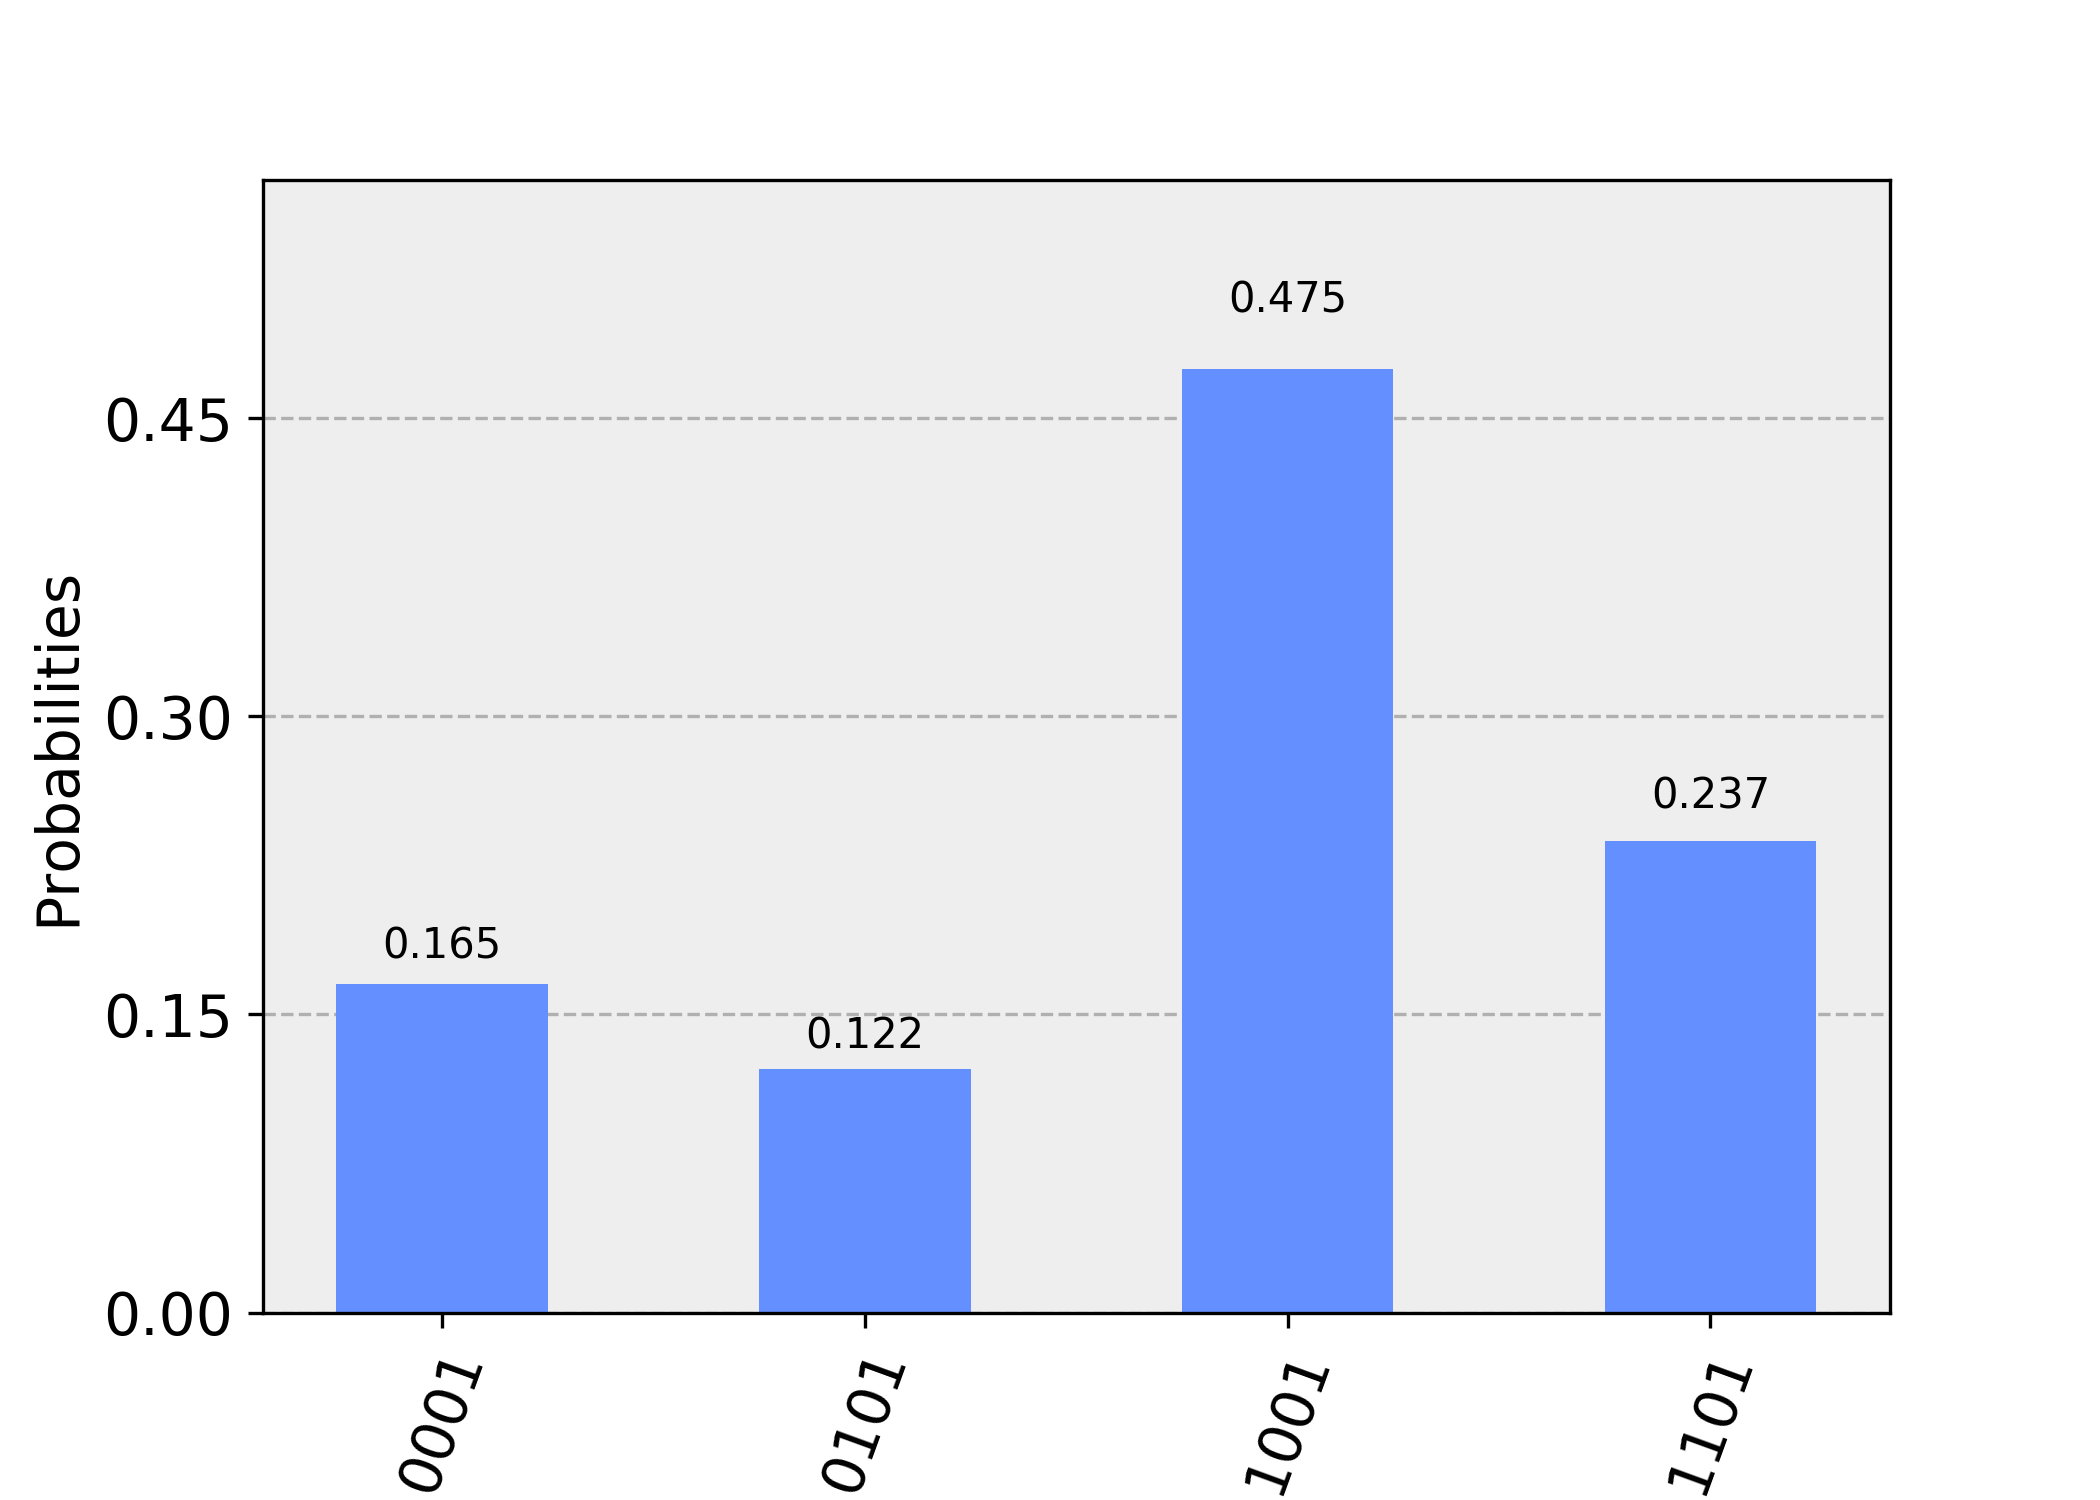
\includegraphics[width=.60\linewidth]{gfx/cluster/Simulated/black}} \quad
    \subfloat[Classe gialla]
    {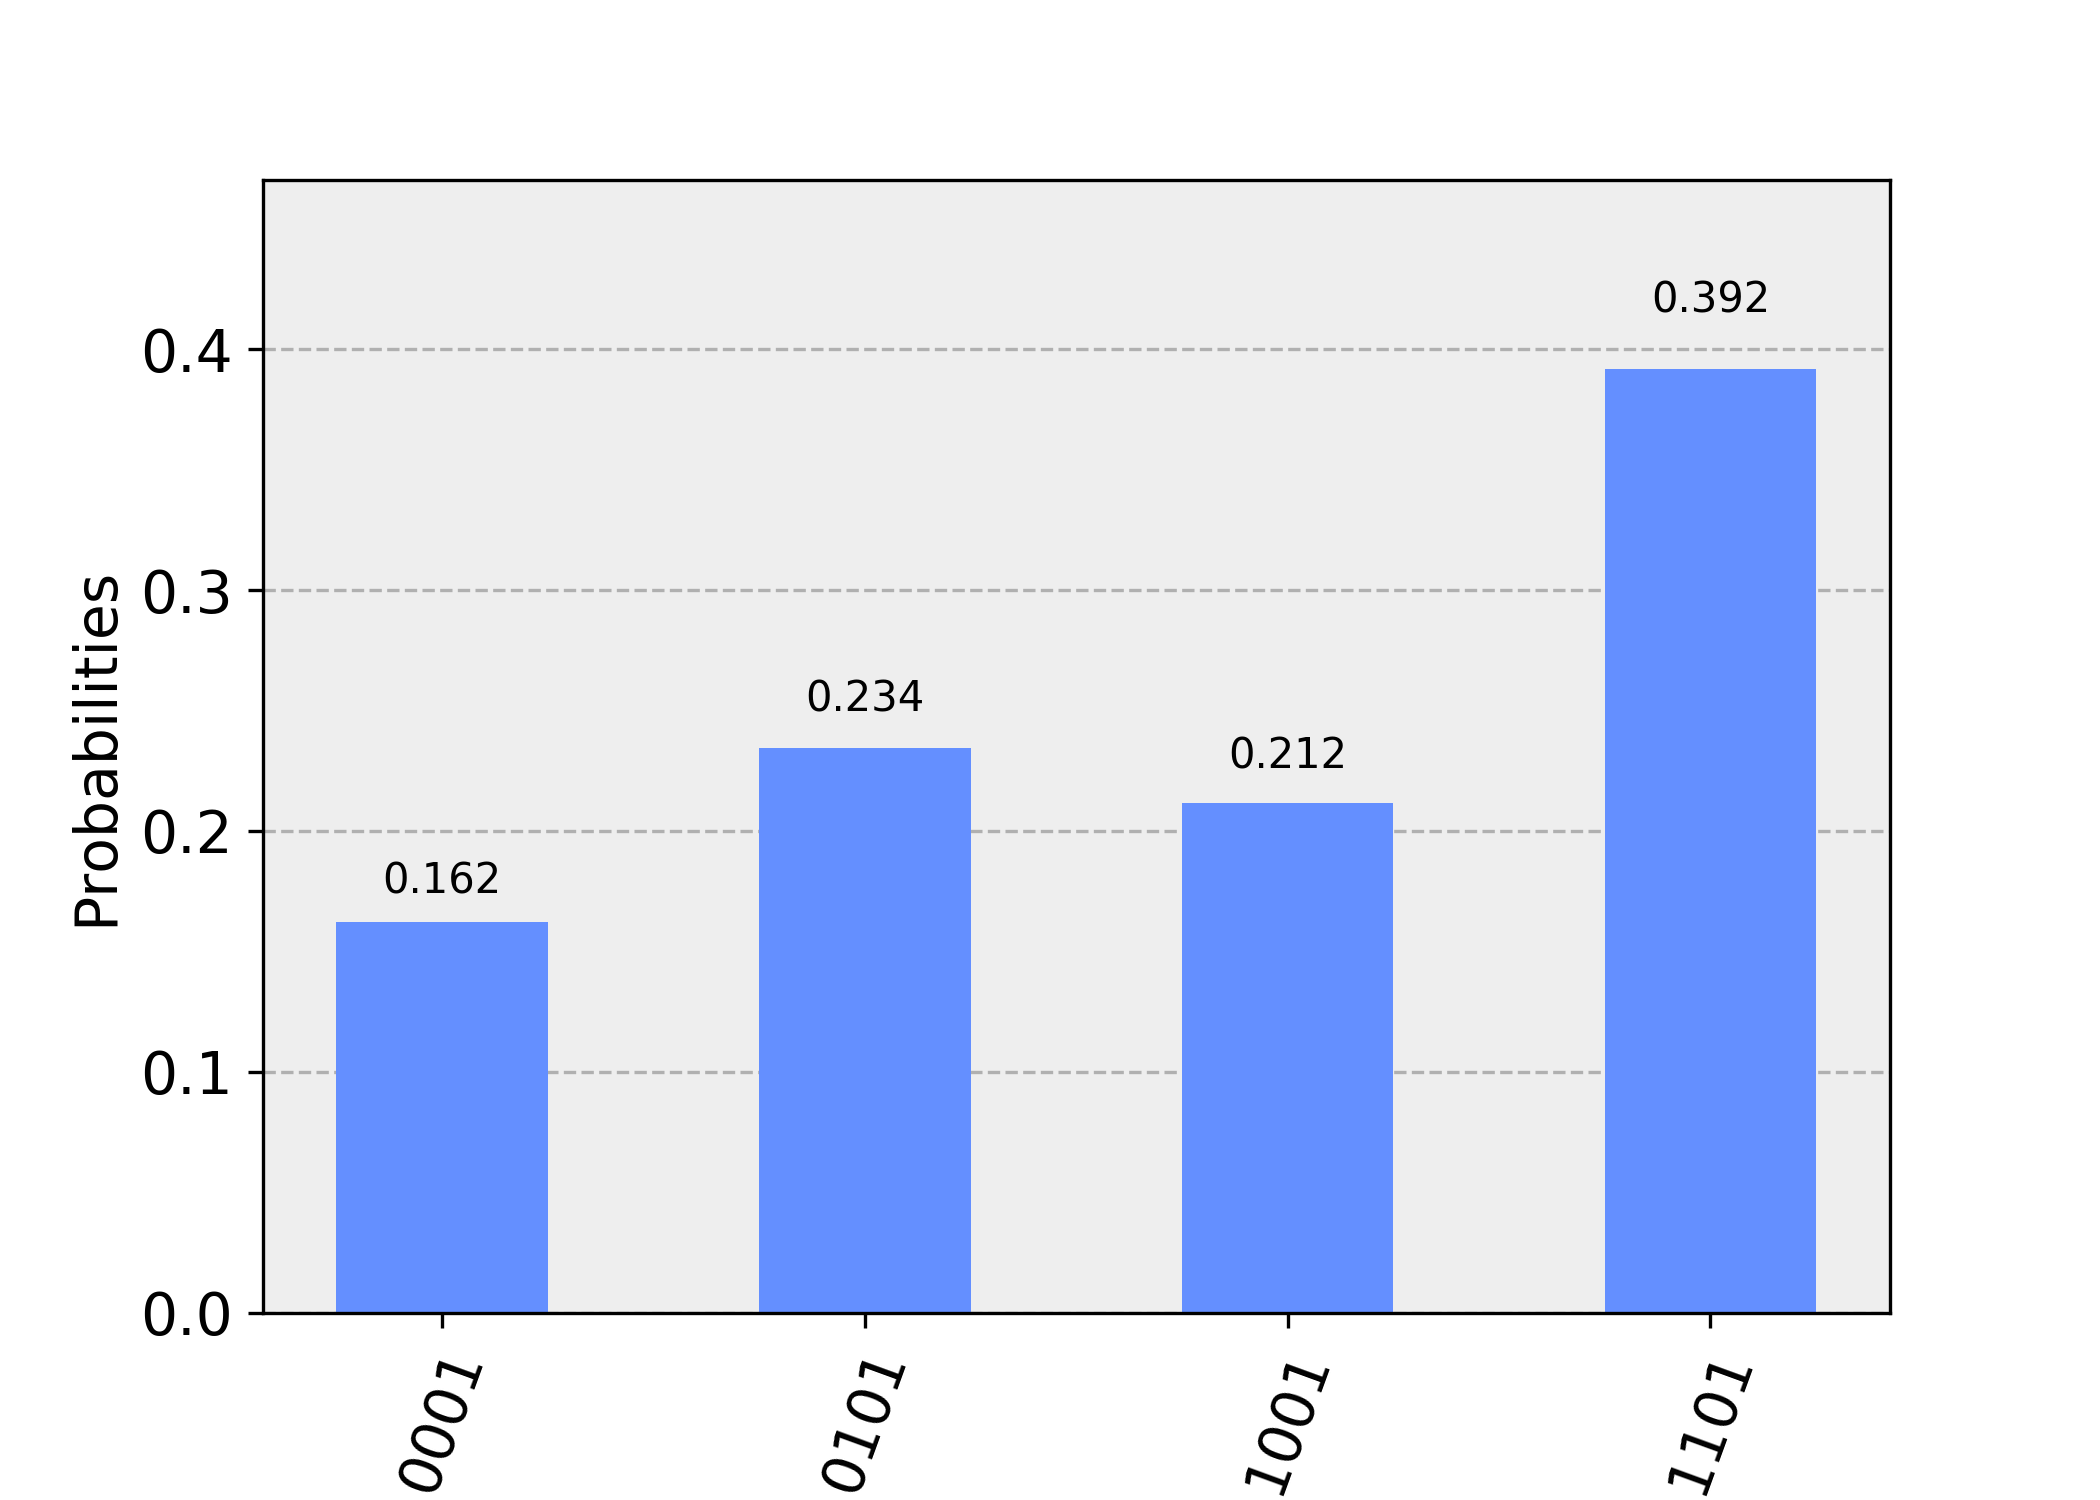
\includegraphics[width=.60\linewidth]{gfx/cluster/Simulated/yellow}}
    \caption{Risultati di simulazione su cluster semplici}
    \label{fig:cluster.simulazione}
\end{figure}

% \begin{figure}[h!]
%     \myfloatalign
%     \subfloat[Classe verde]
%     {\includegraphics[width=.45\linewidth]{gfx/cluster/Real/green}} \quad
%     \subfloat[Classe blu]
%     {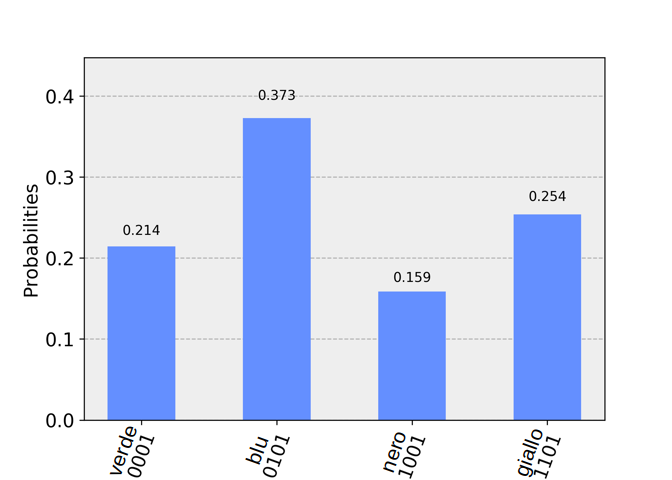
\includegraphics[width=.45\linewidth]{gfx/cluster/Real/blue}} \\
%     \subfloat[Classe nera]
%     {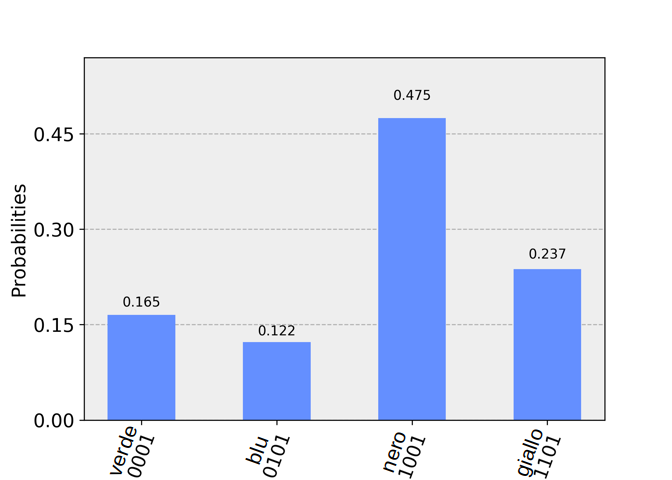
\includegraphics[width=.45\linewidth]{gfx/cluster/Real/black}} \quad
%     \subfloat[Classe gialla]
%     {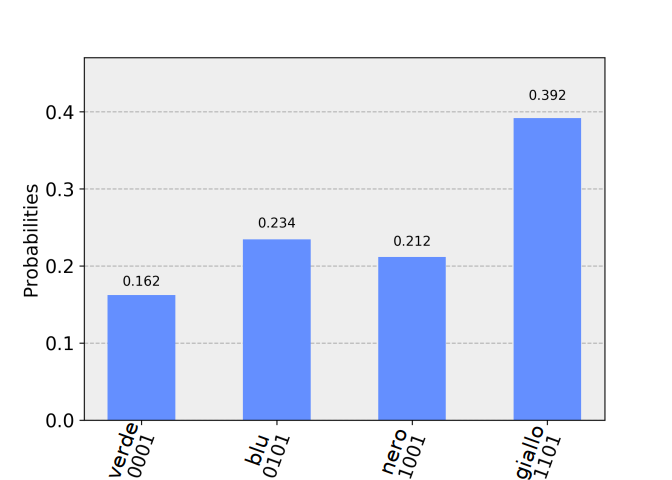
\includegraphics[width=.45\linewidth]{gfx/cluster/Real/yellow}}
%     \caption{Risultati di esecuzione reale su cluster semplici}
%     \label{fig:cluster.esecuzione}
% \end{figure}

